%==============================================================
%  Master Thesis - Main File
%  Compile with: pdflatex -> biber -> pdflatex -> pdflatex
%  (or simply run latexmk, see README)
%==============================================================
\documentclass[
    12pt,
    a4paper,
    oneside,          % two-sided printing; use 'oneside' for screen-only
    openany,        % openright chapters start on right-hand page
    numbers=noenddot,
    bibliography=totoc,
    listof=totoc,
    english            % change to 'ngerman' for a German thesis
]{scrbook}

%--- Configuration (packages, settings, custom commands) ------
%==============================================================
%  Preamble - packages and global settings
%==============================================================

%--- Encoding and language ------------------------------------
\usepackage[utf8]{inputenc}      % source encoding (redundant on modern TeX, harmless)
\usepackage[T1]{fontenc}         % proper font encoding / hyphenation
\DeclareUnicodeCharacter{03BB}{\ensuremath{\lambda}}  % allow raw "λ" in text (e.g. λ-point)
\usepackage{babel}               % language taken from documentclass option
\usepackage{csquotes}            % context-sensitive quotation marks (needed by biblatex)

%--- Fonts ----------------------------------------------------
\usepackage{lmodern}
\usepackage{microtype}           % improved justification and kerning

%--- Mathematics ----------------------------------------------
\usepackage{amsmath}
\usepackage{amssymb}
\usepackage{mathtools}
\usepackage{physics}             % \dv, \pdv, \ket, \bra, \abs, \norm, ...
\usepackage{siunitx}             % \SI{}{}, \si{}, aligned units
\sisetup{
    separate-uncertainty = true,
    per-mode             = symbol,
    range-phrase         = {\text{--}}
}
\DeclareSIUnit{\torr}{Torr}      % not a built-in siunitx unit
\DeclareSIUnit{\groove}{grooves} % not a built-in siunitx unit
\DeclareSIUnit{\bar}{bar}        % re-declare to silence siunitx deprecation warning
\DeclareSIUnit{\ppsi}{psi}        % psi is the letter

%--- Graphics and tables --------------------------------------
\usepackage{graphicx}
\graphicspath{{figures/}}
\usepackage{booktabs}            % \toprule, \midrule, \bottomrule
\usepackage{tabularx}
\usepackage{multirow}
\usepackage{subcaption}          % subfigures
\usepackage[font=small,labelfont=bf]{caption}

\usepackage{tikz}
\usetikzlibrary{arrows.meta,calc,shadings}

% ------------------------------- colours ------------------------------
% Ultraslow centrifuge pulse-shaper diagram (Methods chapter)
\definecolor{cred}{RGB}{227,30,36}
\definecolor{cblue}{RGB}{40,50,150}
\definecolor{cviolet}{RGB}{145,40,145}
\definecolor{cgreen}{RGB}{140,200,80}
\definecolor{ccyan}{RGB}{40,175,225}
\definecolor{cpurple}{RGB}{150,35,145}
\definecolor{cpink}{RGB}{237,20,150}
\definecolor{stagegreen}{RGB}{0,166,81}
\definecolor{stageblue}{RGB}{63,72,204}
\definecolor{plateA}{RGB}{237,60,40}
\definecolor{plateB}{RGB}{247,160,30}

% ---------------------------- optics macros ---------------------------
% \optmirror{coordinate}{direction of surface NORMAL in deg}{length}
\newcommand{\optmirror}[3]{%
  \begin{scope}[shift={(#1)},rotate={#2-90}]
    \fill[black] ({-#3/2-0.035},-0.155) rectangle ({#3/2+0.035},0.010);
    \shade[draw=black,line width=0.3pt,bottom color=black!70,top color=black!3]
      ({-#3/2},-0.015) rectangle ({#3/2},0.075);
  \end{scope}}

% \optgrating{coordinate}{direction of surface NORMAL in deg}{length}
\newcommand{\optgrating}[3]{%
  \begin{scope}[shift={(#1)},rotate={#2-90}]
    \fill[black] ({-#3/2-0.04},-0.20) rectangle ({#3/2+0.04},0.015);
    \foreach \k in {0,...,6}{%
      \shade[draw=black,line width=0.25pt,left color=black!8,right color=black!45]
        ({-#3/2+\k*#3/7},0.0) rectangle ({-#3/2+\k*#3/7+0.5*#3/7},0.105);}
  \end{scope}}

% \optpbs{coordinate}{edge length}
\newcommand{\optpbs}[2]{%
  \begin{scope}[shift={(#1)}]
    \shade[draw=black,line width=0.4pt,left color=black!6,right color=black!40]
      ({-#2/2},{-#2/2}) rectangle ({#2/2},{#2/2});
    \draw[black,line width=0.4pt] ({-#2/2},{#2/2}) -- ({#2/2},{-#2/2});
  \end{scope}}

% \optbeam{A}{B}{half width at A}{half width at B}{colour on the -90 side}{colour on the +90 side}
% The gradient is perpendicular to the propagation direction (spectrally dispersed beam).
\newcommand{\optbeam}[6]{%
  \pgfmathanglebetweenpoints{\pgfpointanchor{#1}{center}}{\pgfpointanchor{#2}{center}}%
  \edef\beamangle{\pgfmathresult}%
  \begin{scope}
    \pgfsetadditionalshadetransform{\pgftransformrotate{\beamangle}}%
    \shade[bottom color=#5,top color=#6,middle color=cviolet]
      ($(#1)!#3cm!90:(#2)$) -- ($(#2)!#4cm!-90:(#1)$) --
      ($(#2)!#4cm!90:(#1)$) -- ($(#1)!#3cm!-90:(#2)$) -- cycle;
  \end{scope}}

\usepackage{wrapfig}

\usepackage{booktabs}
\usepackage{xcolor}
\usepackage{array}

% fixed-width, left-aligned paragraph column
\newcolumntype{P}[1]{>{\raggedright\arraybackslash}p{#1}}

% small grey label (incl. citation) top-left, value centered below
\newcommand{\lab}[1]{{\footnotesize\color{gray}#1}}
\newcommand{\pcell}[2]{%
  \lab{#1}\par\vspace{2pt}%
  {\centering #2\par}\vspace{1pt}%
}

% base grid: 6 equal columns; spans absorb the intervening rules/padding
\newlength{\basecol}\setlength{\basecol}{1.75cm}
\newlength{\spanII}  \setlength{\spanII} {\dimexpr 2\basecol + 2\tabcolsep +  \arrayrulewidth\relax}
\newlength{\spanIII} \setlength{\spanIII}{\dimexpr 3\basecol + 4\tabcolsep + 2\arrayrulewidth\relax}
\newlength{\spanVI}  \setlength{\spanVI} {\dimexpr 6\basecol +10\tabcolsep + 5\arrayrulewidth\relax}

\setlength{\extrarowheight}{2pt}
%--- Layout ---------------------------------------------------
\usepackage[
    a4paper,
    inner = 3.0cm,
    outer = 2.5cm,
    top   = 2.5cm,
    bottom= 2.5cm
]{geometry}
\usepackage{setspace}
\onehalfspacing
\usepackage{scrhack}             % KOMA compatibility fixes
\usepackage{scrlayer-scrpage}    % headers/footers (KOMA)
\pagestyle{scrheadings}
\clearpairofpagestyles
\renewcommand*{\chaptermark}[1]{\markboth{\thechapter\ #1}{}}
\renewcommand*{\sectionmark}[1]{\markright{\thesection\ #1}}
\ihead{\leftmark\ \textbullet\ \rightmark}   % Kapitel • Section
\ohead{\pagemark}  


%--- Brand colours and accent ---------------------------------
\definecolor{ubcblue}{HTML}{002145}   % UBC Blue
\definecolor{rwthblue}{HTML}{00549F}  % RWTH Blau 100%
\definecolor{rwthcyan}{HTML}{8EBAE5}  % RWTH Blau 50% (light)
\colorlet{accent}{rwthblue}           % <- single switch for the accent colour

%--- Coloured caption labels (Fig. 1, Table 1, ...) -----------
\captionsetup{labelfont={bf,color=accent}}
\captionsetup[figure]{name=Fig.}
\captionsetup[table]{name=Tab.}
% To use different colours for figures and tables instead, replace the
% line above with the two lines below:
% \captionsetup[figure]{labelfont={bf,color=rwthblue}}
% \captionsetup[table]{labelfont={bf,color=ubcblue}}

%--- Boxed environments (textbook-style asides) ---------------
\usepackage[most]{tcolorbox}

\usepackage[hidelinks]{hyperref}
\hypersetup{
    pdftitle    = {Master Thesis},
    pdfauthor   = {Your Name},
    colorlinks  = false
}
\usepackage[capitalise,noabbrev]{cleveref}  % \cref, \Cref

%--- Bibliography ---------------------------------------------
\usepackage[
    backend  = biber,
    style    = numeric-comp,     % swap for 'phys' if biblatex-phys is installed
    sorting  = none,             % order of appearance
    giveninits = true
]{biblatex}

%--- Misc -----------------------------------------------------
\usepackage{lipsum}              % placeholder text; remove in final version

%--- Glossary and acronyms ------------------------------------
\usepackage[toc,acronym,nonumberlist,nopostdot]{glossaries}
\setacronymstyle{long-short}
\makeglossaries
%==============================================================
%  Custom commands and shortcuts
%==============================================================


%--- Frequently used physics notation -------------------------
% Note: the 'physics' package already provides \expval, \abs, \norm, \ket, ...
\newcommand{\Jrot}{J}                          % rotational quantum number
\newcommand{\Brot}{B}                           % rotational constant
\newcommand{\tHe}{\ce{^3He} }
\newcommand{\fHe}{\ce{^4He} }

\newcommand{\OCS}{\ce{OCS}\textsuperscript{\ref{tab:ocs-params} }}
\newcommand{\CSS}{\ce{CS2}\textsuperscript{\ref{tab:cs2-params} }}
\newcommand{\NOD}{\ce{(NO)2}\textsuperscript{\ref{tab:no2-params} }}

%--- Units frequently used (siunitx) --------------------------
\DeclareSIUnit{\wavenumber}{\per\centi\meter}   % cm^-1

%--- Editorial helpers (remove in final version) --------------
\newcommand{\todo}[1]{\textcolor{red}{[TODO: #1]}}
\newcommand{\ins}[1]{\textcolor{green}{[#1]}}

%--- Textbook-style aside / info box --------------------------
% Usage: \begin{aside}{Title} ... text ... \end{aside}
% Indented from the left, faint background, accent left rule,
% bold accent-coloured title line. Breaks across pages.
\newtcolorbox{aside}[1]{%
    enhanced, breakable, sharp corners,
    colback = accent!4,                              % faint background tint
    colframe = accent,
    boxrule = 0pt, leftrule = 2pt,                   % accent bar on the left only
    left = 1em, right = 1em, top = 0.7em, bottom = 0.7em,
    width = \dimexpr\linewidth-1.8em\relax,          % narrower than text...
    flush right,                                      % ...indented on the left
    before skip = 1em, after skip = 1em,
    before upper = {{\bfseries\color{accent}#1}\par\smallskip}
}

\loadglsentries{frontmatter/glossary}

%--- Bibliography database ------------------------------------
\addbibresource{bibliography/references.bib}

%==============================================================
\begin{document}
%==============================================================

%--- Front matter (roman page numbers) ------------------------
\frontmatter
\pagenumbering{roman}

%==============================================================
%  Title page
%==============================================================
\begin{titlepage}
\centering

% --- Header banners: UBC left, RWTH right --------------------
% Adjust the logo size in ONE place here:
\newlength{\logoheight}\setlength{\logoheight}{2.4cm}   % <- Größe hier
\noindent\hspace*{-1.2cm}%
\makebox[\dimexpr\textwidth+2.4cm\relax]{%
  
\includegraphics[height=\logoheight]{ubc_banner.png}\hspace{0.3cm}
  
\includegraphics[height=\logoheight]{rwth_banner.pdf}}%
\par
\vspace{1.8cm}

% --- University / department (optional, remove if redundant) -
{\scshape\large University of British Columbia \par}
{\scshape RWTH Aachen University \par}
\vspace{1.5cm}

% --- Title ---------------------------------------------------
{\huge\bfseries Rotational Dynamics of Molecules in\\ Superfluid Helium Nanodroplets\\ Driven by an Optical Centrifuge \par}
\vspace{0.5cm}
{\large Master Thesis \par}
\vspace{2.0cm}

% --- Author --------------------------------------------------
{\Large Sören Eike Mahr \par}
\vspace{0.5cm}
{\normalsize Matriculation number: 466949 \par}
\vspace{2.0cm}

% --- Supervision ---------------------------------------------
\begin{tabular}{rl}
First examiner:  & Prof.\ Dr.\ Markus Ternes \\
Second examiner: & Prof.\ Dr.\ Valery Milner \\
\end{tabular}

\vfill
% --- Date ----------------------------------------------------
{\large Submitted on \today \par}

\end{titlepage}

\cleardoublepage

%==============================================================
%  Abstract
%==============================================================
\chapter*{Abstract}
\addcontentsline{toc}{chapter}{Abstract}

% English abstract
\todo{abstract.}

\cleardoublepage

\tableofcontents
\cleardoublepage

% Optional lists (comment out if not needed)
\listoffigures
\cleardoublepage
\listoftables
\cleardoublepage

\printglossary[type=\acronymtype,title={List of Abbreviations}]
\printglossary[title={Glossary}]
\cleardoublepage

%--- Main matter (arabic page numbers) ------------------------
\mainmatter
\pagenumbering{arabic}

%==============================================================
\chapter{Introduction}
\label{ch:introduction}
%==============================================================

% Motivation, state of the art, and objectives of the thesis.
% Introduce superfluid helium nanodroplets as a matrix, the concept of
% controlling molecular rotation, and the optical centrifuge as a tool.

\section{Motivation}
\label{sec:motivation}
\todo{Why study molecular rotation in superfluid helium nanodroplets.}

\section{State of the Art}
\label{sec:state-of-the-art}
\todo{Existing work on laser-controlled rotation and doped droplets~\cite{example}.}

\section{Objectives and Outline}
\label{sec:outline}
\todo{Research question and chapter-by-chapter outline of the thesis.}

%==============================================================
\chapter{Theoretical Background}
\label{sec:theory}
%==============================================================

\section{Superfluid Helium}
\label{sec:superfluidity}
\todo{Write about why helium stays liquid and the difference 3He and 4He}
\subsection{Bulk Superfluid Helium}
As already shortly introduced in the motivation of this work, after there was experimental evidence that something strange is happening at lower temperatures in liquid helium \cite{keesomNewMeasurementsSpecific1935a, kapitzaViscosityLiquidHelium1938, allenFlowLiquidHelium1938}, theorists like Landau and later Feynman tried explaining the unusual behavior. Based on London's proposed connection between superfluidity and Bose-Einstein condensation  \cite{londonLPhenomenonLiquidHelium1938}, Tisza developed the two-fluid model \cite{tiszaTransportPhenomenaHelium1938}. He stated that in liquid helium below the $\lambda$ point, "atoms in the lowest energy state do not take part in the dissipation of momentum" thus the system should consist of two quantum-statistical populations:
\begin{itemize}
    \item frictionless component $|$ atoms in their lowest energy state
    \item viscous component $|$ atoms in excited states
\end{itemize}
A few years later Landau derives his theory of superfluidity helium II. He starts his first paper \cite{terhaar46THEORYSUPERFLUIDITY1965, landauTheorySuperfluidityHelium1941} with the statement that atoms in their ground state would scatter off excited atoms thereby dismissing Tisza's idea partially. We will later see that the macroscopic idea of two-fluids will persist. 
Landau is convinced that a strongly interacting many-body system cannot be understood in terms of single-atom states. Instead of describing the liquid as a collection of individual particles, he adopts a field-theoretic description, going from the particle operators $\hat{\mathbf r}_a, \hat{\mathbf p}_a$ to the field operators
\begin{equation}
\begin{aligned}
    \mathrm{Mass-density:} \qquad &\hat\rho(\mathbf R)=\sum_a m_a\,\delta(\hat{\mathbf r}_a-\mathbf R) \\
    \mathrm{Momentum-density:}\qquad &\hat{\mathbf j}(\mathbf R)=\frac{1}{2}\sum_a\big[\hat{\mathbf p}_a\,\delta(\hat{\mathbf r}_a-\mathbf R)+\delta(\hat{\mathbf r}_a-\mathbf R)\,\hat{\mathbf p}_a\big]\\
    \mathrm{Velocity:} \qquad &\hat{\mathbf v}(\mathbf R)=\frac{1}{2}\big[\hat\rho^{-1}(\mathbf R)\,\hat{\mathbf j}(\mathbf R)+\hat{\mathbf j}(\mathbf R)\,\hat\rho^{-1}(\mathbf R)\big]
\end{aligned}
\end{equation}
with $\mathbf R$ an arbitrary point in space. All the physics now follows from the commutation relations of these fields, in particular the velocity–velocity relation
\begin{equation}
    [\hat v_i(\mathbf R_1),\hat v_k(\mathbf R_2)] = \frac{\hbar}{i}\,\delta(\mathbf R_1-\mathbf R_2)\;\hat\rho^{-1}(\mathbf R_1)\,(\operatorname{curl}\hat{\mathbf v})_{ik},
\qquad (\operatorname{curl}\hat{\mathbf v})_{ik}=\frac{\partial \hat v_k}{\partial x_i}-\frac{\partial \hat v_i}{\partial x_k}
\end{equation}
where the velocity only commutes when the curl vanishes. From this he stresses: a state that does not possess curl will maintain curlless under the Hamiltonian, i.e. a liquid started in potential flow could never develop a vortex.

\begin{comment}
and the relation obtained by taking the curl of the curl-density commutator
\begin{equation}
    [(\operatorname{curl}\hat{\mathbf v})(\mathbf R_1),\,\hat\rho(\mathbf R_2)]=0 .
\end{equation}
So $\operatorname{curl}\hat{\mathbf v}$ always commutes with the density, but — as Landau stresses — its components commute neither with each other nor with $\hat{\mathbf v}$, and therefore $\operatorname{curl}\hat{\mathbf v}$ does not commute with the Hamiltonian and is not a conserved quantity. The single exception is the case in which $\operatorname{curl}\hat{\mathbf v}$ vanishes over the whole volume: then the right-hand side of the velocity–velocity relation vanishes, and $\operatorname{curl}\hat{\mathbf v}$ commutes with $\hat\rho$, with $\hat{\mathbf v}$, and hence with the Hamiltonian — indeed with any functional of these two fields. In Landau's words, $\operatorname{curl}\hat{\mathbf v}$ is conserved if it is zero. The content of the argument is that the condition
\begin{equation}
    \mathcal H_{\mathrm{pot}}=\big\{\,|\Psi\rangle : \operatorname{curl}\hat{\mathbf v}(\mathbf R)\,|\Psi\rangle=0 \quad \forall\,\mathbf R\,\big\}
\end{equation}
is preserved by the dynamics: if $|\Psi\rangle$ is irrotational, so are $\hat\rho\,|\Psi\rangle$, $\hat{\mathbf v}\,|\Psi\rangle$ and $e^{-i\hat Ht/\hbar}\,|\Psi\rangle$. Since $\hat H$ is hermitian, the orthogonal complement is invariant as well, so
\begin{equation}
    \mathcal H=\mathcal H_{\mathrm{pot}}\oplus\mathcal H_{\mathrm{vort}},\qquad \mathcal H_{\mathrm{vort}}:=\mathcal H_{\mathrm{pot}}^{\perp},
\end{equation}
and the two sectors do not combine: a liquid started in potential flow could never develop a vortex.
\end{comment}

Landau then argues, by analogy with angular momentum, whose components also commute only when they all vanish, and whose spectrum is therefore discrete rather than continuous down to zero, that no states exist with $\operatorname{curl}\hat{\mathbf v}$ non-zero but arbitrarily small. There is thus no continuous transition between potential and vortex motion, and the spectrum must consist of two superimposed continua, the vortex one beginning a finite interval $\Delta$ above the potential ground state.  The elementary excitations of the potential spectrum are the phonons, $\varepsilon = cp$; those of the vortex spectrum he names *rotons*, $\varepsilon = \Delta + p^2/2\mu$.

Landau's theory is phenomenological, and remarkably successful as such. Given the spectrum, everything  (specific heat, normal density, second sound, the critical velocity) follows from the single idea that a strongly interacting quantum liquid must be described by the collective excitations of the whole system rather than by the states of its individual atoms. That idea is correct, and it has outlived every technical detail of the paper that introduced it.

But the spectrum itself is put in by hand. $\Delta$ and $\mu$ are fitted to the measured specific heat, not derived. The model breaks down if one asks what the liquid actually does. Starting in the ground state of $\hat H_\mathrm{pot}$, a liquid in potential flow can never acquire a roton. Yet the thermodynamics presupposes an equilibrium population $e^{(-\Delta/k_BT)}$, which can only establish itself if rotons are freely created and destroyed at the walls. Landau abandoned the two-branch picture in 1947, on the ground that two intersecting curves are unsatisfactory plus new experimental data, and replaced them by a single curve, linear at first, then through a maximum and dipping through a minimum. 

What is missing is a route from the helium atoms themselves to the curve $\varepsilon(p)$. Feynman supplies it, and does so by rehabilitating the very hypothesis Landau's opening paragraph dismisses: London's proposal that superfluidity is a consequence of Bose statistics. In his 1954 paper \cite{feynmanAtomicTheoryTwoFluid1954} he derives Landaus physics from ground up. The start is the excited state wave function
\begin{equation}
    \Psi = \big[\sum_i{f(\mathbf r_i)\big] \phi}
\end{equation}
where $f(\mathbf r_i)$ is some function of position and $\phi$ is the ground-state wave function of the system obeying Bose statistics. For two atoms as $\mathbf r_i \rightarrow \mathbf r_j$ the factor $\phi$ becomes small. This implements the physical behavior of the liquid. $\sum_i{f(\mathbf r_i)}$ is a spatial modulation pattern acting on the ground state. Additionally, $\langle\Psi | \phi\rangle = 0$ is a requirement for the excited state which imposes some conditions on $f$. Feynman inserts this trial wavefunction $\Psi$ into the variational principle and minimizes the energy with respect to $f$ at fixed momentum. The variational estimate becomes the dispersion relation
\begin{equation}
    E(k) = \frac{\hbar^2k^2}{2m S(k)}
\end{equation}
where $S(k)$ is the structure factor of the liquid, a quantity that can be measured directly (neutron or x-ray scattering).  The numerator is just the kinetic energy of a free atom of momentum $\hbar k$; all the many-body physics is contained in the factor $1/S(k)$, which reduces to $1$ for an uncorrelated system, so that $E(k) \rightarrow \hbar^2k^2/2m$. In the liquid, however, he finds $S(k) = \hbar k / 2m c$ for small $k$ which gives the same phonon dispersion relation that Landau had found too ($E(k) = \hbar k c$ with $c$ being the velocity of sound). For intermediate $k \approx 2\pi / a$, around the interatomic spacing, the structure factor possesses a maximum and the excitation energy is correspondingly suppressed there, producing the roton minimum where $E(k) \approx \Delta + \hbar^2(k-k_0)^2/2\mu$. The actual, measured dispersion relation with its phonon and roton part is displayed in \figref{fig:dispersion_relation}. Although this closely resembles Landau's phenomenological result, in Feynman's treatment the roton is built from the same density-modulation ansatz as the phonon and carries no intrinsic angular momentum, so despite the name inherited from Landau, it is not identified with vortex motion. That is to say, that Feynman gives an upper bound on the energy $E(k)$ for every momentum i.e. for the energy gap $\Delta$. Most importantly it automatically explains the one branch picture -> phonons and rotons are quasi particles of the same spectrum. In his original paper the estimated energy gap $\Delta \approx 18 \mathrm{K}$ turned out to be way higher than Landaus fitted $9.6\mathrm{K}$. In a later paper \cite{feynmanEnergySpectrumExcitations1956} Feynman and Cohen brought this number closer ($11.5 \mathrm{K}$) by introducing backflow.

The liquid at $T = 0\, \mathrm{K}$ occupies the ground state $\hat H |0\rangle = E_0 |0\rangle$ with no quasi particle excitations thermally populated. To excite a quasi particle in the superfluid an external perturbation has to add energy and momentum $E_{\mathrm{excited}} = E_0 + \varepsilon(p)$. Now imagine an object of mass $M$ moving through the liquid with velocity $V$. If it creates an excitation with $\varepsilon(p)$ afterwards it moves with $V'$ so
\begin{equation}
    MV = M\mathbf V' + \mathbf p \Rightarrow \mathbf V' = \mathbf V -\frac{\mathbf p}{M}
\end{equation}
and the energy
\begin{equation}
    \frac{1}{2}MV^2 = \frac{1}{2}MV'^2 + \varepsilon(p) \Rightarrow \varepsilon(p) = \mathbf V\mathbf p - \frac{p^2}{2M}.
\end{equation}
So an excitation can be created only if 
\begin{equation}
    V \ge \frac{\varepsilon(p)+ p^2/2M}{p}
\end{equation}
which for macroscopic objects ($M \rightarrow \infty$ ) gives this gives an energy loss of $\varepsilon (p) = V p$ for a given $p$. The criterion for the Landau velocity
\begin{equation}
    V_c = \min_{p} \frac{\varepsilon(p)}{p}.
    \label{eq:landau_velocity}
\end{equation}
He formulated that there is no viscosity for objects moving slower than $V_c$ because for an object moving at velocity $V < V_c$ supplying some momentum $p$ there will never be enough energy $\varepsilon (p)$ to create an elementary excitation. Formula \eqnref{eq:landau_velocity} can be displayed as the linear function with the smallest slope touching the dispersion curve (displayed orange in \figref{fig:dispersion_relation}).

\begin{figure}
    \centering

    \begin{minipage}[t]{0.48\textwidth}
        \centering
        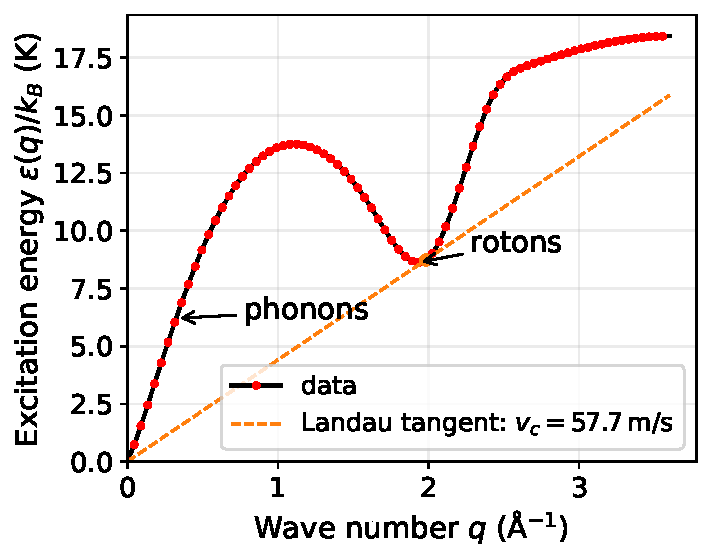
\includegraphics[width=\linewidth]{02_theory/dispersion_curve.pdf}
        \caption{Dispersion relation of superfluid helium around $1K$ from neutron scattering measurements (values taken from \cite{donnellyObservedPropertiesLiquid1998}) }
        \label{fig:dispersion_relation}
    \end{minipage}
    \hfill
    \begin{minipage}[t]{0.48\textwidth}
        \centering
        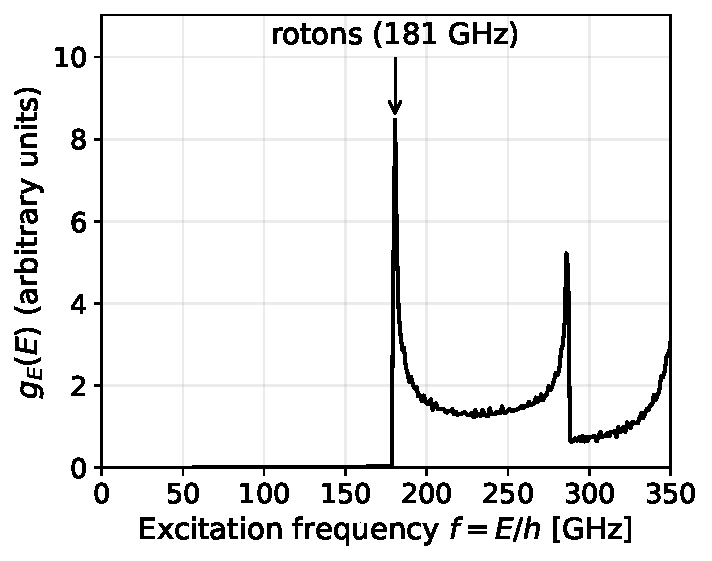
\includegraphics[width=\linewidth]{02_theory/helium_density_of_states_GHz.pdf}
        \caption{For simplicity, the graph of the DOS is calculated by looking at finite intervals $[q_i, q_{i+1}]$ that spares us the pain of calculating the singularities.}
        \label{fig:dos}
    \end{minipage}

\end{figure}
Let's now calculate the density of states of the superfluid. We start by assuming the liquid is in a cubic box of volume $V = L^3$. The volume of a state in three-dimensional momentum space is then
\begin{equation}
    \left(\frac{2\pi}{L}\right)^3  = \frac{(2\pi)^3}{V}
\end{equation}
Because liquid helium is isotropic the excitation energy only depends on the magnitude $q = | \mathbf q |$ and the number of states inside a small volume shell can be written as
\begin{equation}
    dN = \frac{4\pi q^2 dq}{(2\pi)^3 / V} = V\frac{q^2}{2 \pi ^2}dq
\end{equation}
The density of states $g_E(E)$ is defined by 
\begin{equation}
    \frac{dN}{V} = \frac{g_E(E)}{V} dE \qquad \mathrm{with} \quad dE = \frac{dE}{dq}dq \Rightarrow dq = \frac{dE}{dE / dq}
\end{equation}
putting everything together yields
\begin{equation}
    \frac{g_E(E)}{V} = \frac{1}{2\pi^2} \frac{q(E)^2}{|\frac{dE}{dq}|}.
\end{equation}
Mind the absolute value here. Because the dispersion can decrease with q this is necessary and also forces us to take a closer look at the density of states. For example, an energy between the roton minimum and the maxon maximum satisfies $E(q_1) = E(q_2) = E(q_3)$. Therefore, all contributions must be added
\begin{equation}
    \frac{g_E(E)}{V}
=
\frac{1}{2\pi^2}
\sum_{q_i:\,E(q_i)=E}
\frac{q_i^2}
{\left|\dfrac{dE}{dq}\right|_{q_i}}
\end{equation}
Another special feature of the superfluid density of states is the behavior at the roton minimum and maxon maximum where $dE/dq = 0$. At these energies $g_E(E)$ diverges, which in condensed matter physics is commonly known as Van Hove singularities. 

In order to establish the first connection to the main topic of this work, i.e. spinning molecules, we display the DOS in units of GHz (\figref{fig:dos}).

\subsubsection{Why there is Dissipation before the Landau velocity}
The excitation spectrum accounts well for the equilibrium behavior of the superfluid: the specific heat, the normal-fluid density, the entropy and the two-fluid thermodynamics all follow from counting the thermally excited phonons and rotons, and the agreement with experiment is good. This is the regime our density of states describes. The picture is more limited, however, once the fluid is set in motion. The critical velocity is not an equilibrium property but a question of how flowing superfluid sheds momentum, and here the spectrum is no longer the whole story.

Whether the Landau velocity is actually reached turns out to depend on the size of the moving object. For microscopic probes, depending on the system, dissipation does set in close to $V_L$, since roton emission is the only channel available. The ion experiments of Allum, McClintock, Phillips and Bowley confirmed this roton-limited threshold and remain a clean experimental test of Landau's criterion in helium \cite{allumBreakdownSuperfluidityLiquid1977}. For macroscopic objects dissipation and viscosity are commonly observed to develop earlier, below $v_L \approx 60\,\mathrm{m/s}$.\cite{mullerCriticalVelocityVortex2022} Feynman himself notes that resistance can set in at velocities a few hundred times smaller than the roton estimate \cite{feynmanChapterIIApplication1955}. Thus there has to be some cheaper mechanism dissipating energy well before $V_L$ is reached.

That cheaper mechanism is the nucleation of quantized vortices, for which Feynman gives an order-of-magnitude estimate in his jet picture \cite{feynmanChapterIIApplication1955}. He considers superfluid issuing from a slot of width $d$ into a reservoir at rest: the jet carries velocity $v$ inside and zero outside, and this discontinuity is a circulation the fluid can only support as discrete quantized vortex lines. Forming them costs energy that must be drawn from the flow's kinetic energy, and equating the two gives a critical velocity of order $v_c \approx 1\,\mathrm{m/s}$  (for a given set of parameters), almost two orders of magnitude below the roton limit.

\subsection{Finite Size Effects}
\label{sec:finite_size}
The physics laid out so far is that of bulk helium, but the following experiments in this theses are performed in nanodroplets, where the finite number of atoms in the system alters the picture. The most important point is that in a droplet the excitation spectrum is not a fixed input. The phonon-maxon-roton curve that we have leaned on throughout emerges only as the system size grows: theoretical calculations find no roton minimum at all in the smallest clusters, only a weak dip near $N \approx 70$, and a curve approaching its bulk depth and position only once a few hundred atoms are present \cite{ramakrishnaCollectiveExcitationsHelium1990, guardiolaExcitedStates4He2001}. The density of states we constructed from that curve is therefore a bulk idealisation that a finite droplet only approaches, and quantities read off it inherit the same size dependence. The Landau velocity is the clearest example: taken as $\min(\epsilon/p)$ over the computed $N = 240$ spectrum it already comes out at $V_L \approx 49\,\mathrm{m/s}$, below the bulk value even at a size where the dispersion otherwise looks nearly bulk \cite{ramakrishnaCollectiveExcitationsHelium1990}. 

Infrared spectroscopy of free rotating molecules in helium droplets consisting of about $10^4$ atoms showed superfluid behavior \cite{grebenevSuperfluiditySmallHelium41998}. A genuine Landau-type critical velocity has since been measured in droplets of only $\sim\!10^3$ atoms \cite{brauerCriticalLandauVelocity2013}. Finite size does not abolish the superfluid behavior our spectrum describes; it sets the scale on which that behavior appears and rescales the quantities that follow from it.

Finite size also governs the cheaper dissipation channel. The quantized vortices that let bulk superfluid shed momentum well below $V_L$ are observed in droplets too. Whether and how this cheaper channel operates in a droplet is an open question. Quantized vortices are not forbidden in small droplets, theory finds stable vortex solutions down to droplets of order $10^2$ atoms \cite{lehmannEnergeticsPossibleFormation2003}, experimentally they have been imaged only in large ones. Gomez and co-workers traced vortices by decorating the cores with silver atoms and found them present only in droplets of  $>300 \, \mathrm{nm}$ diameter \cite{gomezTracesVorticesSuperfluid2012} and the x-ray diffraction images of vortex lattices were likewise taken in droplets of $10^8 -10^{11}$ atoms \cite{gomezShapesVorticitiesSuperfluid2014}. 
All of these lie far above the size regime of the work presented in this thesis. System size in our setup ranges from $10^3-10^4$ helium atoms per droplet.  Which does not directly imply that dissipation in our system can't come from vortex nucleation. 

\todo{Talk about ripplons in finite size systems??}

\section{Molecule Interactions}
\label{sec:molecule_interaction}

A complete quantum-mechanical description of a molecule is generally very complex because it must account for the coupled motion of all electrons and nuclei. This problem can be much simplified using the Born-Oppenheimer approximation. Based on the nuclei being much heavier than the electrons, in a given system, coordinates of the nuclei remain fixed while the wave function is governed by the dynamic electron positions. This makes it possible to handle the total energy as a sum of non interacting terms
\begin{equation}
    E_{\mathrm{total}} = E_{\mathrm{electronic}} + E_{\mathrm{vibrational}} + E_{\mathrm{rotational}} + E_{\mathrm{nuclear\ spin}}.
    \label{eq:energy_sum}
\end{equation}
Because the characteristic level spacing scales like
\begin{equation}
    \Delta E_{\mathrm{rot}} \ll \Delta E_{\mathrm{vib}} \ll \Delta E_{\mathrm{el}},
    \label{eq:level_spacing}
\end{equation}
in further approximation for diatomic molecules we can use the rigid rotor model. This model assumes that the system is well enough described by looking at the rotational energy of the molecule
\begin{equation}
    \hat{H}_{\mathrm{rot}} \lvert \psi \rangle = E_{\mathrm{rot}} \lvert \psi \rangle
    \label{eq:rigid_rotor_se}
\end{equation}
whit $\hat{H}_{\mathrm{rot}} = \hat J^2 / 2I$ where $\hat J$ is the total angular momentum operator and $I$ the moment of intertia. In the basis of spherical harmonics $Y_J^{M_J}(\theta, \Phi)$ with the total angular momentum quantum number $J = 0, 1, 2,3,..$ and the projection onto the quantization axis $M_J = 0, \pm 1, \pm 2, .., \pm J$ the $2J+1$ degenerate eigenvalues of the rigid rotor are
\begin{equation}
    E_{rot}(J) = BJ(J+1).
    \label{eq:rigid_rotor_energy}
\end{equation}
The constant in that expression is called rotational constant
\begin{equation}
    B = \frac{\hbar^2}{2I}
    \label{eq:rotational_constant}
\end{equation}
and provides the measure for level spacing depending on the moment of inertia of the molecule.

\begin{aside}{Centrifugal Distortion}
In the rigid-rotor approximation, the distances between the atoms are assumed to remain constant during molecular rotation. Real molecules, however, are not perfectly rigid. As the rotational angular momentum increases, the effective centrifugal force slightly stretches the molecular bonds. This increases the moment of inertia and consequently lowers the rotational energy relative to the rigid-rotor prediction \cite{mcnabRotationalSpectroscopyTheory2017}.

The rotational energies can be represented as an expansion in powers of $J(J+1)$, corresponding to the rotational part of the Dunham expansion. Retaining only the leading centrifugal-distortion correction gives
\begin{equation}
    E_J = B J(J+1) - D\left[J(J+1)\right]^2
    \label{eq:centrifugal_distortion}
\end{equation}
where $B$ is the rotational constant and $D$ is the centrifugal-distortion constant.
\end{aside}

\subsection{Molecules in Helium Nanodroplets}

A molecule embedded in a superfluid helium nanodroplet is not an isolated rotor. The attractive van der Waals interaction between the dopant and the surrounding helium creates a local density enhancement, a solvation shell, in the first few atomic layers around the molecule. For a sufficiently anisotropic potential energy surface, part of this shell is rigidly bound to the molecular frame and follows the molecular orientation adiabatically during rotation \cite{grebenevRotationalSpectrumSingle2000, choiInfraredSpectroscopyHelium2006a}. The rotating object is therefore the molecule plus a fraction of the helium it drags along, which increases the effective moment of inertia and correspondingly reduces the rotational constant.

Rotational spectroscopy of different molecules in \fHe droplets, showed that the spectrum remains that of a free rotor, sharp resolvable lines with the same symmetry, but with rescaled $B$ constant. Typical reductions are a factor of $2 - 4$ relative to the gas phase value \cite{toenniesSuperfluidHeliumDroplets2004a}. ``Kicking'' the molecules and observing dynamics of higher rotational states confirmed the spectroscopy values including the rescaling of the centrifugal-distortion constant $D$. Instead of $D$ describing the bond stretching of a free rotating molecule, in this case it is connected to the attached helium shell spreading out and increasing the moment of inertia \cite{chatterleyRotationalCoherenceSpectroscopy2020}. The already in section \ref{sec:state-of-the-art} mentioned experiments by the Stapelfeldt group showed, that for example for \OCS $D_\mathrm{He} \approx 7.3 \times 10^3 \, D_\mathrm{gas}$. Plotting the transition frequency $\Delta E_{J \rightarrow J+2}$ as a function of $J$ reveals a striking consequence of the enhanced distortion constant: the transition frequency does not increase monotonically but reaches a maximum and then decreases (see \figref{fig:centrifugal_wall}), so that beyond this point a state of higher angular momentum is connected by a transition of lower frequency. This eventually results in an unphysical decrease of rotational frequency with higher $J$. In this thesis the turning point is referred to as the centrifugal wall. Further, with the kick experiments it was not possible to resolve what actually happens when approaching the centrifugal wall. Accordingly, the maximum energy for \gls{css} was $E(J=10) \approx 66 \, \mathrm{GHz}$ and for \OCS $E(J=5) \approx 57 \, \mathrm{GHz}$, both way below the roton energy.

\begin{figure}[htbp]
    \centering
    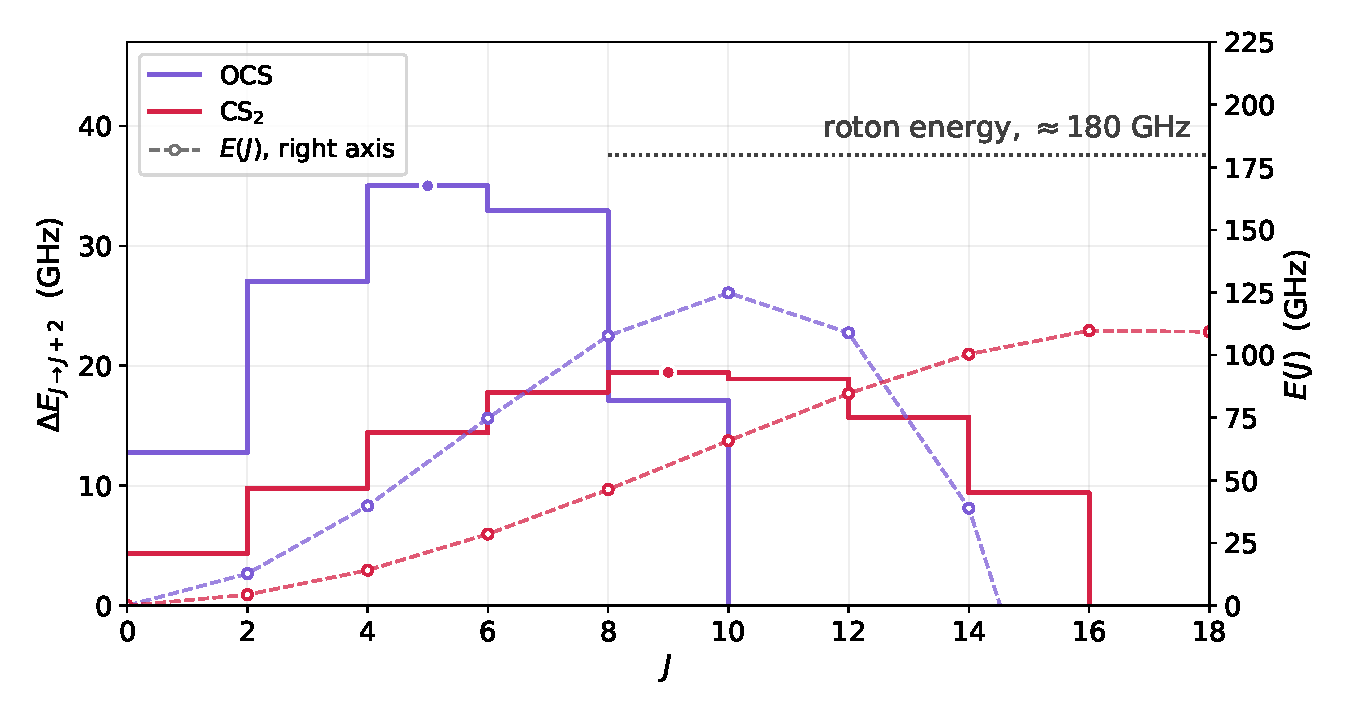
\includegraphics[width=\textwidth]{02_theory/cfg_wall_roton.pdf}
    \caption{Breakdown of the rigid rotor with centrifugal distortion model in superfluid helium. \OCS and \CSS transition energies displaying the "centrifugal wall", where with the next $J \rightarrow J +2$ step the transition needs less energy. The molecules rotational energy is plotted on the right-hand side, consequently also showing unphysical behavior for higher rotational states. Note that for both molecules only the even ladder is displayed - due to lack of symmetry, \OCS can also develop the uneven ladder with $\Delta J = 2$ \cite{ianThesis, nielsenLaserInducedAlignmentMolecules2022}. The wall for \CSS appears to be $J = 8 \rightarrow 10$ ($19.4\, \mathrm{GHz}$), for \OCS $J = 5 \rightarrow 7$ ($35.4\, \mathrm{GHz}$)} 
    \label{fig:centrifugal_wall}
\end{figure}

This raises some important questions:
Is it possible to shed the helium shell and recover the gas phase rotational constants? Can we even bring the molecules closer to the energy regime of roton creation ($\approx 180 \, \mathrm{GHz}$)?

All these previous experiments observe field free dynamics of the molecules. Intuitively, if I have a strong enough rotating laser field that holds my molecule, I should be able to spin to higher angular momentum states.

\subsection{Molecules in an Electric Field}
\label{sec:molecules_in_efield}

With these questions raised, let's look at what happens to a molecule when it is acted upon by an electric field. First we need to define the interaction between the laser field and the molecule. In the limit of large photon number, treating the field quantum mechanically yields the same dynamics as in the classical case \cite{kremsMoleculesElectromagneticFields2019} chapter 4.8.3. This lets us write the Hamiltonian of the system within the electric dipole approximation\footnote{the spatial variation of the electromagnetic field is negligible across the system} as
\begin{equation}
    \hat H = \hat H^{(0)} + \hat H^{(1)}
    \label{eq:hamiltonian_split}
\end{equation}
where $\hat H^{(0)}$ describes the unperturbed dynamics and $\hat H^{(1)} = -\hat{\vec\mu}\cdot\vec\varepsilon$, with the electric dipole moment operator $\hat{\vec\mu} = \sum_a q_a \hat{\vec r}_a$ and the electric field vector $\vec\varepsilon$, implements the classical perturbation. Note that this coupling is exactly linear in the field: the Hamiltonian contains no term of higher order in $\vec\varepsilon$. Nonlinear dependency of the energy on the field must therefore come from the wavefunction dependence on the electric field. The energy of the system can be expanded in a Taylor series about the field-free case, where summation over repeated Cartesian indices $i,j,k \in \{x,y,z\}$ is implied:
\begin{equation}
    E(\vec\varepsilon) = E(0) + \left(\frac{\partial E}{\partial\varepsilon_i}\right)_{\!0}\varepsilon_i + \frac{1}{2}\left(\frac{\partial^2 E}{\partial\varepsilon_i\,\partial\varepsilon_j}\right)_{\!0}\varepsilon_i\varepsilon_j + \frac{1}{6}\left(\frac{\partial^3 E}{\partial\varepsilon_i\,\partial\varepsilon_j\,\partial\varepsilon_k}\right)_{\!0}\varepsilon_i\varepsilon_j\varepsilon_k + \cdots
    \label{eq:energy_expansion}
\end{equation}
Subscript $0$ denotes evaluation at zero field. Following \cite{atkinsMolecularQuantum}, because of the Hellmann--Feynman theorem, the variation of the energy takes the form
\begin{equation}
    \frac{\partial E}{\partial\varepsilon_i} = \left\langle \Psi(\vec\varepsilon)\left|\frac{\partial \hat H}{\partial\varepsilon_i}\right|\Psi(\vec\varepsilon)\right\rangle = -\langle\hat\mu_i\rangle
    \label{eq:hellmann_feynman}
\end{equation}
where $\Psi(\vec\varepsilon)$ is an eigenstate of the perturbed system. This now implies that the derivatives actually have physical meaning. Identifying
\begin{equation}
    \mu_{0i} \equiv -\left(\frac{\partial E}{\partial\varepsilon_i}\right)_{\!0}, \qquad \alpha_{ij} \equiv -\left(\frac{\partial^2 E}{\partial\varepsilon_i\,\partial\varepsilon_j}\right)_{\!0}, \qquad \beta_{ijk} \equiv -\left(\frac{\partial^3 E}{\partial\varepsilon_i\,\partial\varepsilon_j\,\partial\varepsilon_k}\right)_{\!0}
    \label{eq:moment_definitions}
\end{equation}
gives rise to the dipole expression
\begin{equation}
    \langle\hat\mu_i\rangle = \mu_{0i} + \alpha_{ij}\varepsilon_j + \tfrac{1}{2}\beta_{ijk}\varepsilon_j\varepsilon_k + \cdots
    \label{eq:dipole_expansion}
\end{equation}
with the permanent dipole moment $\mu_{0i}$, the polarizability $\alpha_{ij}$ and the hyperpolarizability $\beta_{ijk}$, of rank one, two and three respectively.

All of these factors can be calculated by perturbation theory with the Hamiltonian in equation \eqnref{eq:hamiltonian_split}. Normally each state (labeled by rotational, vibrational and electronic quantum number) has its own energy shift; given the energy of optical photons, the electronic contribution is the main drive for the energy shift, therefore the polarizability \cite{kremsMoleculesElectromagneticFields2019} chapter 4.6. Consequently, the molecule frame properties $\alpha_\perp$ and $\alpha_\parallel$ (with respect to the molecules axis) are constant for all the rotational levels that we are interested in. The dependence of the interaction on the rotational state enters not through $\alpha$ itself, but through the orientation of the molecular axis relative to the field.

For the next steps we disregard $\mathcal{O}(\varepsilon^4)$ in $E$. The effective potential energy surface induced by the electric field can be written as
\begin{equation}
    U(\vec\varepsilon) = E(\vec\varepsilon) - E(0) = -\mu_{0i}\varepsilon_i - \tfrac{1}{2}\alpha_{ij}\varepsilon_i\varepsilon_j - \tfrac{1}{6}\beta_{ijk}\varepsilon_i\varepsilon_j\varepsilon_k
    \label{eq:potential_static}
\end{equation}
The expressions above were obtained for a static field. For a monochromatic non-resonant field, time-dependent perturbation theory yields an energy shift of the same functional form, with the coefficients evaluated at the driving frequency. For a linearly polarized pulse with a slowly varying envelope, we insert $\vec\varepsilon(t) = \varepsilon_0(t)\cos(\omega t)\,\vec e_{\mathrm{pol}}$, where $| \vec e_{\mathrm{pol}} | = 1$. Since the optical frequency also greatly exceeds both the rotational frequencies and the inverse pulse duration, $\omega\gg\omega_{\mathrm{rot}},\tau^{-1}$, the rotational motion experiences only the potential averaged over one carrier period. Averaging, knowing that $\langle\cos^{2n+1}(\omega t)\rangle = 0$ for $n \in \mathbb{N}_0$ and $\langle\cos^{2}(\omega t)\rangle = \tfrac12$, removes all terms of odd order in the field and leaves
\begin{equation}
    U(t) = -\frac{1}{4}\varepsilon_0^2(t)\;\vec e_{\mathrm{pol}}^{\,\mathrm{T}}\boldsymbol\alpha^{\mathrm{lab}}\vec e_{\mathrm{pol}}.\footnote{Matrix notation $\vec e_{\mathrm{pol}}^{\,\mathrm{T}}\boldsymbol\alpha\vec e_{\mathrm{pol}}$ equals the index notation $\sum_{i,j} \alpha_{ij}\,e_i\,e_j$}
    \label{eq:potential_cycle_averaged}
\end{equation}
In the molecule-fixed frame the polarizability tensor for a linear molecule is diagonal and can be written as $\boldsymbol\alpha^{\mathrm{mol}} = \mathrm{diag}(\alpha_\perp, \alpha_\perp, \alpha_\parallel)$ with $\alpha_\parallel$ being the polarizability along the axis of the molecule. The orientation of the molecule axis in the laboratory frame, where $\theta$ is the polar angle measured from the laboratory $z$-axis and $\varphi$ the azimuth angle in the $x$--$y$ plane, is given by
\begin{equation}
    \vec n = \begin{pmatrix} \sin\theta\cos\varphi \\ \sin\theta\sin\varphi \\ \cos\theta \end{pmatrix}.
    \label{eq:molecular_axis}
\end{equation}
With $\Delta\alpha = \alpha_\parallel - \alpha_\perp$ we get $
    \boldsymbol{\alpha}^{\mathrm{mol}}
    =
    \alpha_\perp \mathbf{I}
    +
    \Delta\alpha\,
    \vec e_{z'}\vec e_{z'}^{\,\mathsf{T}}$, where $\vec e_{z'}$ is the $z$-unit vector in the molecule frame. Using the rotational transformation $R$ (explained in \cite{zareAngularMomentumUnderstanding1989}), the polarizability tensor in the lab frame can be written as
\begin{equation}
    \boldsymbol{\alpha}^{\mathrm{lab}} = 
\mathbf{R}\,
\boldsymbol{\alpha}^{\mathrm{mol}}\,
\mathbf{R}^{\mathsf{T}} = \alpha_{\perp}\mathbf{I} + \Delta\alpha\, \vec{n}\left(\vec{n}\right)^{\mathrm{T}}. \footnote{Disclaimer: Derivation done with the help of AI (see appendix \ref{sec:ai})}
    \label{eq:polarizability_lab}
\end{equation}
Using the effective polarizability, i.e. the projection of the tensor onto the polarization axis $\vec e_{\mathrm{pol}}$, we end up with the following expression for the potential
\begin{equation}
    U(t) = -\frac{1}{4}{\varepsilon}_0(t)^2 \left[ \alpha_{\perp} + \Delta\alpha\,(\vec n\cdot \vec e_{\mathrm{pol}})^2 \right].
    \label{eq:potential_effective}
\end{equation}
Note that $U$, besides the intensity envelope, only depends on the angle between the molecular axis and the instantaneous polarization direction. Since the experiments described in this work use a polarization that rotates in a plane, it is natural to take $\vec e_z$ along the rotation axis and let the polarization lie in the $x$--$y$ plane at azimuth $\Phi$,
\begin{equation}
    \vec e_{\mathrm{pol}}(t) = \begin{pmatrix} \cos\Phi(t) \\ \sin\Phi(t) \\ 0 \end{pmatrix},
    \label{eq:polarization_vector}
\end{equation}
which gives
\begin{equation}
    U(\theta,\varphi,t) = -\frac{1}{4}\varepsilon_{0}^{2}(t)\left[ \alpha_{\perp} + \Delta\alpha\, \sin^{2}\theta\, \cos^{2}\!\left(\varphi-\Phi(t)\right) \right]
    \label{eq:potential_rotating}
\end{equation}
and we can define $U_0 = \frac{\varepsilon_0^2 \Delta \alpha}{4}$.

\subsubsection{Pendular States}

Now that we have the interaction potential for a linear molecule in a non-resonant electric field, the part missing is the description of the rotor. As shown earlier in this section we can use the rigid rotor Hamiltonian $\hat H_{\mathrm{rot}}$ \eqnref{eq:rigid_rotor_se} to describe free rotation. The in-field system follows the time-dependent Schrödinger equation with $\hat{H}_{\mathrm{field\,dressed}} = \hat{H}_{\mathrm{rot}} + U$,
\begin{equation}
    i\hbar \frac{\partial \Psi_{\mathrm{rot}}(t)}{\partial t} = \left( B\hat{J}^{2} - \frac{\varepsilon_{0}^{2}(t)}{4}\left[ \alpha_{\perp} + \Delta\alpha\,\sin^{2}\theta\,\cos^{2}(\varphi - \Phi) \right] \right) \Psi_{\mathrm{rot}}(t),
    \label{eq:tdse_field_dressed}
\end{equation}
where the time dependence of $U$ only lives in the envelope, i.e. the polarization direction $\vec e_{\mathrm{pol}}$ is constant.
Taking a closer look at the Hamiltonian, the only part that is not diagonal in the basis of spherical harmonics is the angular factor of the polarizability term. Rewriting it gives (similar to \cite{larsenLaserInducedAlignment})
\begin{equation}
    \sin^{2}\theta\,\cos^{2}(\varphi-\Phi) = \sqrt{\frac{4\pi}{9}}\,Y_{00} \;-\; \frac{1}{2}\sqrt{\frac{16\pi}{45}}\,Y_{20} \;+\; \frac{1}{4}\sqrt{\frac{32\pi}{15}}\left[ Y_{22}\,e^{-2i\Phi} + Y_{2,-2}\,e^{+2i\Phi} \right]. \footnote{Disclaimer: Calculation done by AI (see appendix \ref{sec:ai})}
    \label{eq:angular_factor_expansion}
\end{equation}
Using this to calculate the coupling $\langle J'M' \rvert \sin^2\theta\cos^2(\varphi-\Phi) \lvert JM\rangle$ imposes the selection rules $\Delta J = 0, \pm2$ and $\Delta M = 0, \pm2$. These are exactly the selection rules of a two-photon Raman transition, which is no coincidence, since the interaction is second order in the field. Though it is to say, that imagining the pendular states as a two photon process is not trivial.

The wavefunction can be expanded in the instantaneous eigenbasis of the field dressed Hamiltonian, giving $\Psi_{\mathrm{rot}}(t) = \sum_n c_n(t)\,|n(t)\rangle$, where the system can either change adiabatically or non-adiabatically. Under a slowly varying Hamiltonian, the population of the instantaneous states will not change in time $|c_n(t)|^2 = |c_n(-\infty)|^2$. Either way, the eigenstates can be written in the field-free rotor basis (following \cite{nielsenLaserInducedAlignmentMolecules2022}) so that 
\begin{equation}
    \Psi_{\mathrm{rot}}(t) = \sum_n c_n(t)\,\sum_{J,M} d^{(n)}_{JM}(t)\,\lvert J M\rangle .
    \label{eq:eigenstate_expansion}
\end{equation}
For a molecule initially in a single rotational state $\lvert J=0, M=0\rangle$ and adiabatic dynamics $|c_0(t)|^2 = 1$, the system will follow one instantanous branch.
Put into words, the field creates a superposition of different angular momentum states. Classically one could imagine the molecules axis librating around the field vector.
Writing the density matrix as
\begin{equation}
    \hat{\rho}(t) = \sum_{JM,\,J'M'} d_{JM}(t)\, d^{*}_{J'M'}(t)\, \lvert J M\rangle \langle J' M'\rvert ,
    \label{eq:density_matrix}
\end{equation}
the diagonal elements yield the population/ probabilities of measuring angular momentum $J$ and the off-diagonal elements display the coherence between different states. These coherences, or in other words the time-dependent relative phases, can provide angular confinement, i.e. molecule alignment to the polarization axis.

Whether the evolution follows a single branch is decided by comparing the rate of change of the Hamiltonian to the energy gaps it must bridge. Transitions between field-dressed states are suppressed as long as \cite{omisteTheoreticalDescriptionAdiabatic2011}
\begin{equation}
    \eta = \frac{\left|\langle m \left| \partial \hat H/\partial t \right| n\rangle\right|}{(E_m - E_n)^2} = \frac{\Delta\alpha}{4}\,\left|\dot\varepsilon_0^2(t)\right|\, \frac{ \left|\langle m|\sin^2\theta\,\cos^2(\varphi-\Phi)|n\rangle\right| }{ \left(E_m-E_n\right)^2 } \ll 1,
    \label{eq:adiabaticity_criterion}
\end{equation}
so the adiabaticity scales with the polarizability anisotropy, the intensity slope and the moment of inertia which enters through the energy difference.

Ortigoso et al. quantified this by solving the pendular problem numerically for a Gaussian envelope, identifying two limiting regimes. In the short-pulse limit, $\sigma\lesssim\hbar/B$, the interaction is non-adiabatic and the pulse leaves behind a rotational wave packet that shows field-free revivals. In the long-pulse limit, $\sigma\gtrsim10\,\hbar/B$, the evolution is truly adiabatic, the alignment follows the pulse envelope, and the initial state is recovered after the pulse.
With the effective in-droplet rotational constants for \OCS and \CSS, one finds $\hbar/B=73\ \mathrm{ps}$ and $218\ \mathrm{ps}$. Adiabatic behavior would thus require $\sigma\gtrsim0.7\ \mathrm{ns}$ for \OCS and $\sigma\gtrsim2.2\ \mathrm{ns}$ for \CSS. Our pulse with \gls{fwhm} duration, $\tau_{\mathrm{FWHM}}=320\ \mathrm{ps}$ ($\sigma\approx192\ \mathrm{ps}$), falls well short of both. In addition, their calculations only demonstrated adiabatic following up to $\Delta\omega=\Delta\alpha\,\varepsilon_{0}^{2}/2B=900$, whereas at a peak intensity of $1\times10^{12}\ \mathrm{W/cm^{2}}$ we reach $\Delta\omega\approx1.1\times10^{3}$ for \OCS and $\approx7.9\times10^{3}$ for \CSS.

We should therefore not expect our system to behave perfectly adiabatically.

\subsubsection{Rotational Ladder climbing}

As stated in the paragraph above, a long linear polarized alignment pulse doesn't transfer angular momentum to the molecule, causing effectively no excitation of rotational states after the field. Since the goal is to have controlled excitation of molecules to measure state lifetimes and the dissipation into superfluid helium, this is where the optical centrifuge comes into play. The rotating linear polarization makes it possible to ``grab'' the molecule and spin it up to higher frequencies. 

Transforming the potential $U$ with its time dependent polarization direction \eqnref{eq:potential_rotating} into the frame co-rotating, gives the rotating-frame Hamiltonian
\begin{equation}
    \hat{\tilde H}(t) = B\hat J^{2} - \hbar\Omega(t)\hat J_{z} - \frac{\varepsilon_0^2(t)}{4}\left[\alpha_\perp + \Delta\alpha,\sin^2\theta\cos^2\varphi\right], \qquad \Omega=\dot\Phi .
    \label{eq:rotating_frame_hamiltonian}
\end{equation}
The polarization is now static, at the price of the term $-\hbar\Omega\hat J_z$. For constant $\Omega$ the Hamiltonian is time-independent, so its eigenstates are the rotating analogs of the pendular states.
With no rotation the in-field Hamiltonian was diagonal in the pendular state basis. The term $-\hbar\Omega\hat J_z$ now generates coupling of the different branches. As $\Omega$ grows, states of large $M$ are pulled down and their energies cross those of the lower $J$ states. The energies of $|J,M\rangle$ and $|J{+}2,M{+}2\rangle$ become degenerate at
\begin{equation}
    \hbar\Omega_{J,J+2} = B(2J+3),
    \label{eq:crossing_condition}
\end{equation}
i.e. at $t_{J,J+2}=B(2J+3)/\hbar\beta$ for a linear chirp $\Omega=\beta t$ (explained in detail in sec. \ref{sec:optical_centrifuge}). The coupling $V_{J,J+2}\propto\Delta\alpha\varepsilon_0^2$ turns each degeneracy into an avoided crossing. The rotational excitation is thus a chain of real two-photon Raman crossings encountered one after another \cite{vitanovAdiabaticExcitationRotational2004}. Only here does the adiabatic branch change character: following it means climbing the ladder $|0,0\rangle\to|2,2\rangle\to|4,4\rangle\to\dots$. Simulating the dynamics of the Hamiltonian in eq. \eqnref{eq:rotating_frame_hamiltonian} yields a good insight into the ladder climbing mechanism, mainly showing that population transfer only happens if the centrifuge frequency exceeds a level crossing (compare \figref{fig:ladder_climbing_simulation}).

\begin{figure}[htbp]
    \centering
    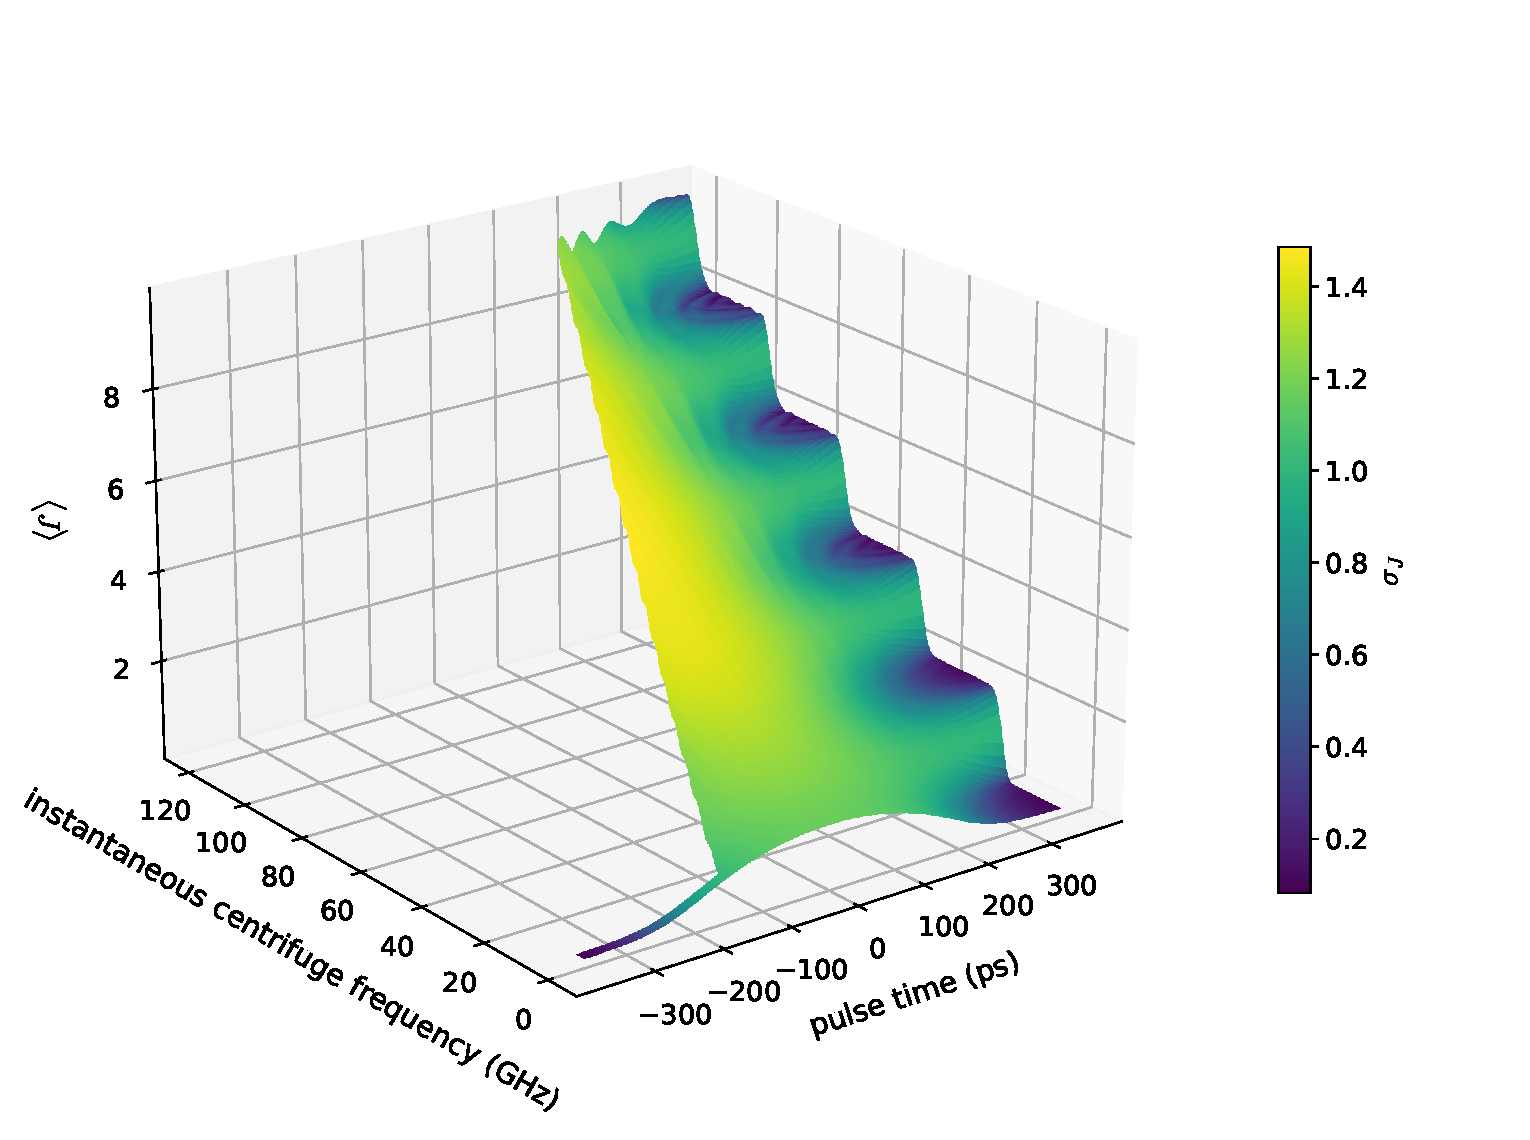
\includegraphics[width=1\textwidth]{02_theory/ocs_gaussian_fan.pdf}
    \caption[]{Simulation\protect\footnotemark ~of the $J$ state distribution of gas-phase \OCS starting in $\vert 0\, 0\rangle$, under an electromagnetic field with $320\, \mathrm{ps}$ FWHM Gaussian envelope and $10^{11}\,\mathrm{W}/\mathrm{cm}^2$ maximum intensity. $\sigma_J$ is standard deviation of the rotational distribution. Different accelerations (ranging from $0 \rightarrow 0 \, \mathrm{GHz}$ to $0 \rightarrow 100 \, \mathrm{GHz}$) during the high intensity part, map out the surface. As expected, for no rotation, the field creates pendular states, i.e. $\langle J \rangle > 0$, stays on the instantaneous branch and returns to the initial state after the field. Only if the rotation frequency exceeded the first transition, the molecule stays in $J = 2$ after the field.}
    \label{fig:ladder_climbing_simulation}
\end{figure}
\footnotetext{Disclaimer: Simulation created with the help of AI (see appendix \ref{sec:ai-cfg})}

Once the intensity has reached its plateau, the rate of change of $\hat{\tilde H}$ is dominated by the chirp, $\partial\hat{\tilde H}/\partial t \simeq -\hbar\dot\Omega\hat J_z$, and the criterion of eq. \eqnref{eq:adiabaticity_criterion} becomes
\begin{equation}
    \eta = \frac{\hbar|\dot\Omega|\left|\langle m|\hat J_z|n\rangle\right|}{\left(E_m-E_n\right)^2} \ll 1 .
    \label{eq:adiabaticity_chirp}
\end{equation}
This is noticable in the simulation, where for higher accelerations the rippels on the surface get more pronounced, displaying the branch hopping/ non-adiabaticity (\figref{fig:ladder_climbing_simulation}).

Whether the excitation really proceeds as the step-by-step ladder and if the criterion in equation \eqnref{eq:adiabaticity_chirp} is a valid measure, depends on how well the individual crossings are separated in time. Armon and Friedland
\cite{armonQuantumClassicalDynamics2017} cast this into two dimensionless parameters built from the sweep time $t_s=1/\sqrt{\beta}$, the drive time $t_d=\hbar/\epsilon$ (with $\epsilon=\Delta\alpha\,\varepsilon_0^2/4$) and the rotational time $t_c=I/\hbar$:
\begin{equation}
    P_1=\frac{\epsilon}{\hbar\sqrt{\beta}},\qquad
    P_2=\frac{2B}{\hbar\sqrt{\beta}} .
    \label{eq:armon_parameters}
\end{equation}
Successive steps are only resolved if $P_2\gg\tfrac14+\tfrac{P_1}{16}$. Below, several states are coupled
at once, the ladder structure washes out, and the dynamics is better described classically as
autoresonance: the molecular axis stays phase-locked in the rotating well and follows $\Omega(t)$.
Capture into autoresonance requires $P_1P_2>1/2$, i.e.
\begin{equation}
    \frac{I\beta}{\epsilon}<2 ,
    \label{eq:autoresonance_condition}
\end{equation}
the torque of the well must exceed what is needed to keep up with the accelerating trap (same scaling as Karczmarek's $I\beta<\epsilon/2\pi$ \cite{karczmarekOpticalCentrifugeMolecules1999}).


\section{The Optical Centrifuge}
\label{sec:optical_centrifuge}

The optical centrifuge was proposed theoretically in 1999 by Karczmarek, Wright, Corkum and Ivanov \cite{karczmarekOpticalCentrifugeMolecules1999} and the first experimental realization followed one year later, in 2000, by Villeneuve, Aseyev, Dietrich, Spanner, Ivanov and Corkum \cite{villeneuveForcedMolecularRotation2000}. Conceptually it is described by an intense linear polarized laser pulse, where the polarization vector is rotating in the plane perpendicular to the propagation direction. The field behavior is realized by superimposing two circular polarized chirped pulses with opposite handedness.

\begin{aside}{Chirped pulses}
An ultrashort laser pulse has a finite spectral bandwidth $\Delta\omega$. For a given spectral amplitude, the pulse is called transform limited when its spectral phase contains no nonlinear frequency dependence. In the time domain, this means that all frequency components have the same group delay and therefore overlap optimally in time. The spectral phase can be expanded in a Taylor series around the central frequency $\omega_0$:
\begin{equation}
    \phi(\omega) = \phi_0 + \phi'(\omega-\omega_0) + \frac{\phi''}{2}(\omega-\omega_0)^2 + \frac{\phi'''}{6}(\omega-\omega_0)^3 +\cdots .
    \label{eq:spectral_phase_taylor}
\end{equation}
Here, $\phi_0$ is the constant phase, $\phi_1$ is the group delay at the central frequency, and $\phi_2$ is the \gls{gdd}. The linear phase term $\phi_1$ shifts the entire pulse in time without changing its temporal shape. The quadratic phase term $\phi_2$, however, makes the group delay frequency dependent:
\begin{equation}
    \tau_g(\omega) = \frac{d\phi}{d\omega} \approx \phi'+\phi''(\omega-\omega_0).
    \label{eq:group_delay}
\end{equation}
Consequently, different frequency components are localized at different times. This produces a linear chirp and broadens the pulse relative to its transform-limited duration.
\end{aside}

We can label the two pulses by $j\in\{R,L\}$, with propagation distances $z_R$ and $z_L$. Instead of introducing a separate time delay, propagation is included directly through the retarded time
\begin{equation}
    u_j(t,z_j)=t-\frac{z_j}{c}.
    \label{eq:retarded_time}
\end{equation}
The temporal phase of each propagating chirped pulse can be written as
\begin{equation}
    \Phi_j(t,z_j) = \omega_{j0}u_j(t,z_j) + \frac{1}{2}\beta_j u_j^2(t,z_j) + \varphi_{j0}.
    \label{eq:time_phase}
\end{equation}
where $\beta_j$ is now the temporal chirp and $\omega_{j} = d\Phi_j/d t$ the instantaneous optical frequency. Assuming a Gaussian envelope in the form of
\begin{equation}
    A_j(t,z_j) = A_0 \exp\left[ -\frac{u_j^2(t,z_j)}{2T_j^2} \right],
    \label{eq:gaussian_envelope}
\end{equation}
the two circular pulses can be written as
\begin{equation}
    \vec E_R(t,z_R) = \frac{A_R(t,z_R)}{\sqrt{2}} \begin{pmatrix} 1\\ i \end{pmatrix} e^{i\Phi_R(t,z_R)} \qquad
    \vec E_L(t,z_L) = \frac{A_L(t,z_L)}{\sqrt{2}} \begin{pmatrix} 1\\ -i \end{pmatrix} e^{i\Phi_L(t,z_L)},
    \label{eq:circular_fields}
\end{equation}
giving $\vec E(t, z_R, z_L) = \vec E_R + \vec E_L$, the linear polarized field vector. This vector is rotating with frequency of
\begin{equation}
    \Omega_{\mathrm{cfg}}=2\pi f_{\mathrm{cfg}} = \frac{1}{2}[\omega_{R}(t) - \omega_{L}(t)].
    \label{eq:fcfg}
\end{equation}

\subsection{Different centrifuge types}
\label{sec:different_centrifuge_types}
\begin{figure}[htbp]
    \centering
    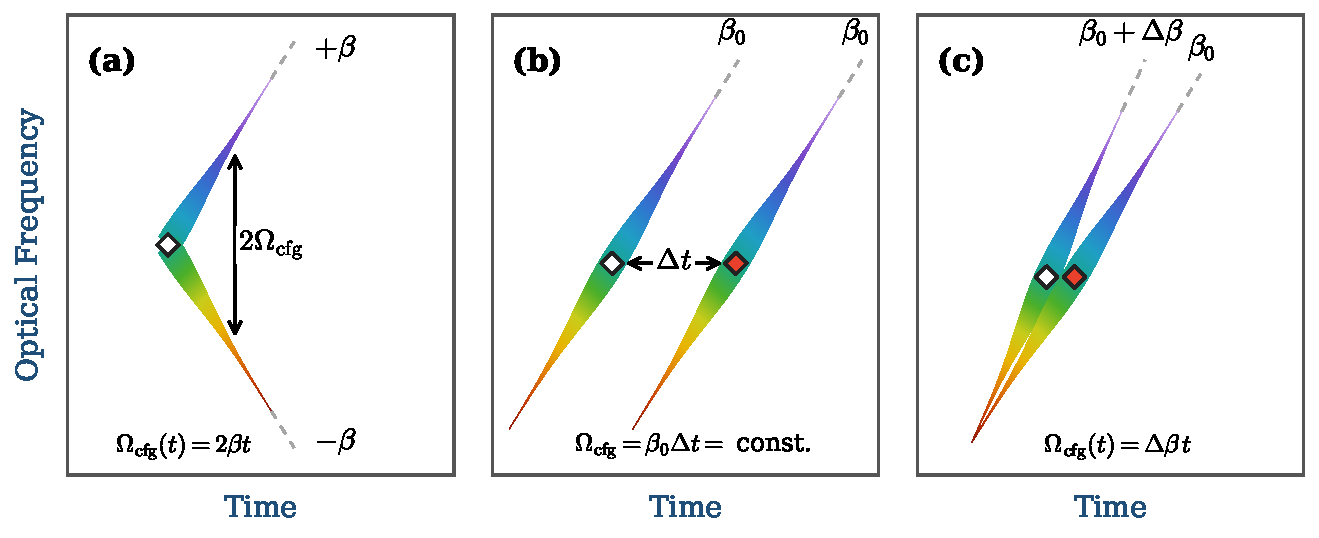
\includegraphics[width=\textwidth]{02_theory/centrifuge_spectrograms.pdf}
    \caption[Different variations of the centrifuge principle using two circular polarized, chirped laser pulses. \textbf{(a)} displays the original \acrshort{cfg} design, achieved by taking a chirped pulse and forming it with a 4f-pulse shaper \cite{macphail-bartleyLaserControlMolecular2020}. A \acrshort{cf} with no angular acceleration, generated by splitting a pulse into a Michelson interferometer and delaying one arm, is seen in \textbf{(b)} \cite{wangOpticalCentrifugeZero2025a}. The \acrshort{us} used in this work is shown in \textbf{(c)}. Additionally to the delay, in this case the other interferometer arm adds chirp to the pulse, yielding slow acceleration \cite{wangUltraslowOpticalCentrifuge2026}.]{Different variations of the centrifuge principle using two circular polarized, chirped laser pulses. \textbf{(a)} displays the original \gls{cfg} design, achieved by taking a chirped pulse and forming it with a 4f-pulse shaper \cite{macphail-bartleyLaserControlMolecular2020}. A \gls{cf} with no angular acceleration, generated by splitting a pulse into a Michelson interferometer and delaying one arm, is seen in \textbf{(b)} \cite{wangOpticalCentrifugeZero2025a}. The \gls{us} used in this work is shown in \textbf{(c)}. Additionally to the delay, in this case the other interferometer arm adds chirp to the pulse, yielding slow acceleration \cite{wangUltraslowOpticalCentrifuge2026}.}
    \label{fig:centrifuge_types}
\end{figure}

With the prerequisite of using oppositely circular polarized, chirped pulses one now can think of various designs. The three most useful variations are shown in \figref{fig:centrifuge_types}, where \textbf{(a)} resembles the initial design of the optical centrifuge \cite{karczmarekOpticalCentrifugeMolecules1999} with $\beta_R = -\beta_L$. For our research, the interesting regime is around $0-180\, \mathrm{GHz}$. A centrifuge of type \textbf{(a)}, depending on the laser used, commonly has a frequency range up to terahertz \cite{korobenkoThesis}, therefore our region of interest occupies only a small portion of the pulse. Decreasing the acceleration in the original centrifuge design is solely possible by decreasing the chirp. This entails, that because of the longer pulse duration, the peak intensity also drops, giving a shallower potential and less alignment to the field, causing the signal-to-noise ratio of the data to drop. Additionally, the physical implementation is restricted by optical components like gratings \cite{macphail-bartleyLaserControlMolecular2020}. Therefore, the Milner research group came up with a new centrifuge design. Take a stretched pulse and use a polarizing beam splitter to send the vertical and horizontal polarized parts into two Michelson interferometer arms. Delay one of them, and you will get the constant frequency centrifuge with zero rotational acceleration (described in detail in \cite{wangOpticalCentrifugeZero2025a}). If you now add a mechanism to slightly change the chirp of one arm, you can tweak the starting and end frequency almost completely independent of the intensity profile. The rotation dynamics of this ultraslow centrifuge (describe in the paper \cite{wangUltraslowOpticalCentrifuge2026} and later in section \ref{sec:usCFG_design}), with the initial chirp $\beta_0$, the additional chirp $\Delta \beta$ and the delay between the two arms $\Delta t$, is described by 

\begin{equation}f_{\mathrm{cfg}}(t) = f_0 + \Delta \beta t / 4 \pi
    \label{eq:f_uscfg}
\end{equation}
with the central frequency $f_0= \beta_0 \Delta t / 4 \pi$. To fully describe the centrifuge pulse, the additional "bandwidth" property $\Delta f_{\mathrm{FWHM}}$ (defined later in section \ref{sec:centrifuge_characterization}) is used.

\subsection{Characterizing the centrifuge}
\label{sec:centrifuge_characterization}

There are multiple ways to characterize the field alignment behavior of this optical tool. The most common way is cross-correlation. For cross- or x-correlation one first has to project the field, that is rotation in the x-y-plane, onto a fixed axis, take the x-axis for example. Using a linear and also x-polarized reference pulse, with a way shorter pulse duration and focussing both on a type-I nonlinear crystal (in our case barium borat, BBO), gives \gls{sfg} (setup explained in \cite{wangUltraslowOpticalCentrifuge2026}). The signal intensity scales with the square of the centrifuge field.
Similar to our actual experimental pump-probe setup, which will be explained later in section \ref{sec:detection}, we scan the delay of the short reference pulse to gain information about the field orientation in time. The measured signal oscillates with twice $f_{\mathrm{cfg}}$ due to the indistinguishable nature of the two x-aligned positions of the field vector per rotation period.

A second, new way to characterize the pulse was developed within the scope of this work. Later we use this method to phase-stabilize the centrifuge (explained in section \ref{sec:detection}). Here, the math is presented to underline what can be done using a spectrometer signal of a likewise x-projected centrifuge. For each arm, the projected field is
\begin{equation}
    E_j(t,z_j) = \frac{A_0}{\sqrt{2}} \exp\left[ -\frac{u_j^2(t,z_j)}{2T_j^2} \right] e^{i\Phi_j(t,z_j)}.
    \label{eq:projected_field}
\end{equation}
Its Fourier transform is evaluated by shifting the integration variable to the retarded time $u_j$. This separates vacuum propagation as a spectral phase factor,
\begin{equation}
    \tilde E_j(\omega,z_j) = e^{-i\omega z_j/c}\tilde E_j(\omega,0).
    \label{eq:propagation_phase}
\end{equation}
The remaining integral is the Fourier transform of a chirped Gaussian. Combining the Gaussian envelope and the quadratic temporal phase gives the complex width
\begin{equation}
    q_j=\frac{1}{T_j^2}-i\beta_j.
    \label{eq:complex_width}
\end{equation}
After completing the square, the integration contour is shifted by a complex constant. This is allowed because $\mathrm{Re}(q_j)=1/T_j^2>0$, so the integrand is exponentially damped, and because the Gaussian integrand is entire. By Cauchy's theorem, the contour can be displaced back to the real axis. The remaining integral is the standard complex Gaussian integral. This gives
\begin{equation}
    \tilde E_j(\omega,z_j) = \frac{A_0}{\sqrt{2}} e^{i\varphi_{j0}} e^{-i\omega z_j/c} \sqrt{\frac{2\pi}{q_j}} \exp\left[ -\frac{(\omega-\omega_{j0})^2}{2q_j} \right].
    \label{eq:spectral_field}
\end{equation}
With the horizontal spectral field being $\tilde E_x(\omega)=\tilde E_R(\omega,z_R)+\tilde E_L(\omega,z_L)$ the spectrometer measures the intensity
\begin{equation}
    I_x(\omega) \propto |\tilde E_R|^2 + |\tilde E_L|^2 + 2\mathrm{Re} \left[ \tilde E_R\tilde E_L^* \right].
    \label{eq:spectrometer_intensity}
\end{equation}
By writing each spectral field as an amplitude and a phase the cross term becomes
\begin{equation}
    2\mathrm{Re} \left[ \tilde E_R\tilde E_L^* \right] = 2|\tilde E_R||\tilde E_L| \cos\Theta(\omega),
    \label{eq:cross_term_spectral}
\end{equation}
which is the origin of the modulation observed on the spectrometer. The phase of the modulation can be written as
\begin{equation}
    \Theta(\omega) = \Theta_0+\Theta_1\omega+\Theta_2\omega^2.
    \label{eq:spectrum_phase}
\end{equation}
Defining $D_j=\frac{1}{T_j^4}+\beta_j^2$ lets us write the constant, linear, and quadratic coefficients as
\begin{equation}
    \Theta_0 = \varphi_{R0}-\varphi_{L0} -\frac{1}{2}\arg(q_Rq_L^*) -\frac{\beta_R\omega_{R0}^2}{2D_R} +\frac{\beta_L\omega_{L0}^2}{2D_L},
    \label{eq:theta0}
\end{equation}
\begin{equation}
    \Theta_1 = \frac{z_L-z_R}{c} + \frac{\beta_R\omega_{R0}}{D_R} - \frac{\beta_L\omega_{L0}}{D_L},
    \label{eq:theta1}
\end{equation}
\begin{equation}
    \Theta_2 = -\frac{\beta_R}{2D_R} + \frac{\beta_L}{2D_L}.
    \label{eq:theta2}
\end{equation}

\subsubsection{Common transform-limited pulse}

In our case both arms originate from the same transform-limited Gaussian pulse with carrier frequency $\omega_{R0}=\omega_{L0}=\omega_0$ and bandwidth $\Delta\lambda_\mathrm{FWHM}$. \gls{gdd} only alters the spectral phase and not the amplitude, so both arms share the same Gaussian envelope $|\tilde E(\Omega)|$ and differ at most by an overall scale set by the beam-splitter ratio. Writing $|\tilde E_R|^2=R\,|\tilde E|^2$ and $|\tilde E_L|^2=L\,|\tilde E|^2$, the spectral intensity becomes
\begin{equation}
    I_x(\Omega)=(R+L)\,|\tilde E(\Omega)|^2\big[\,1+V\cos\Theta(\Omega)\,\big],
    \label{eq:spectral_intensity_common}
\end{equation}
with the fringe visibility $V$
\begin{equation}
    V=\frac{2\sqrt{RL}}{R+L}\le 1.
    \label{eq:visibility}
\end{equation}
For balanced arms ($R=L$, i.e. $V=1$) this reduces to $4|\tilde E|^2\cos^2(\Theta/2)$; an imbalance lowers $V$, so the fringe minima no longer reach the background but instead follow a second, lower Gaussian envelope $(R+L)(1-V)|\tilde E|^2$.
With a common carrier frequency, the three coefficients of Eq.~\eqnref{eq:spectrum_phase} combine, so that with the detuning $\Omega\equiv\omega-\omega_0$, the spectral phase reduces to
\begin{equation}
    \Theta(\Omega) = \Theta_0' - \tau\,\Omega + \frac{1}{2}(\phi''_R - \phi''_L)\,\Omega^2 ,
    \label{eq:spectrum_phase_common}
\end{equation}
where we use the condensed constant $\Theta_0'=\varphi_{R0}-\varphi_{L0}-\tfrac12\arg(q_Rq_L^*)-\tau\omega_0$, the relative arm delay $\tau=(z_R-z_L)/c$ and GDD $\phi''_j = -\beta_j/D_j$.

\subsubsection{Reconstructing the pulse in time}

We start from the inverse $q$-parameter, whose real part is the transform-limited bandwidth and whose imaginary part is the GDD,
\begin{equation}
    \frac{1}{q_j} = a - i\,\phi''_j , \qquad a \equiv \mathrm{Re}\frac{1}{q_j} = \frac{4\ln 2}{\Delta\omega_\mathrm{FWHM}^2}.
    \label{eq:inverse_q}
\end{equation}
Inverting and identifying real and imaginary parts with $q_j = 1/T_j^2 - i\beta_j$,
\begin{equation}
    q_j = \frac{1}{a - i\phi''_j} = \frac{a + i\,\phi''_j}{a^2 + \phi''^2_j},
    \label{eq:q_inverted}
\end{equation}
gives the stretched duration and the temporal chirp rate,
\begin{equation}
    \frac{1}{T_j^2} = \mathrm{Re}(q_j) = \frac{a}{a^2+\phi''^2_j},
    \label{eq:duration}
\end{equation}
\begin{equation}
    \beta_j = -\,\mathrm{Im}(q_j) = -\frac{\phi''_j}{a^2+\phi''^2_j}.
    \label{eq:beta_gdd}
\end{equation}
Converting Eq.~\eqnref{eq:duration} to an intensity FWHM via $T_{j,\mathrm{FWHM}}^2 = 4\ln 2\,T_j^2 = 4\ln 2\,(a^2+\phi''^2_j)/a$ and using $4\ln 2/a = \Delta\omega_\mathrm{FWHM}^2$,
\begin{equation}
    T_{j,\mathrm{FWHM}}^2 = \Delta\omega_\mathrm{FWHM}^2\,(a^2 + \phi''^2_j) = T_{\mathrm{TL},\mathrm{FWHM}}^2 + \big(\phi''_j\,\Delta\omega_\mathrm{FWHM}\big)^2,
    \label{eq:B}
\end{equation}
with the transform-limited duration $T_{\mathrm{TL},\mathrm{FWHM}} = 4\ln 2/\Delta\omega_\mathrm{FWHM}$. Equation~\eqnref{eq:B} solved for the dispersion reads
\begin{equation}
    |\phi''_j| = \frac{\sqrt{T_{j,\mathrm{FWHM}}^2 - T_{\mathrm{TL},\mathrm{FWHM}}^2}}{\Delta\omega_\mathrm{FWHM}}.
    \label{eq:phi}
\end{equation}
Equation~\eqnref{eq:B} also yields the denominator of Eq.~\eqnref{eq:beta_gdd} directly, $a^2 + \phi''^2_j = T_{j,\mathrm{FWHM}}^2/\Delta\omega_\mathrm{FWHM}^2$, so that inserting Eq.~\eqnref{eq:phi} into Eq.~\eqnref{eq:beta_gdd} gives the chirp rate purely in terms of the two measured widths,
\begin{equation}
    |\beta_j| = \Delta\omega_\mathrm{FWHM}\, \frac{\sqrt{T_{j,\mathrm{FWHM}}^2 - T_{\mathrm{TL},\mathrm{FWHM}}^2}}{T_{j,\mathrm{FWHM}}^2}
    \label{eq:chirp_from_widths}
\end{equation}
where $\Delta\omega_\mathrm{FWHM}$ follows from the spectrum and $T_{j,\mathrm{FWHM}}$ from the cross-correlation of arm $j$.
As already seen the chirp rates and arm delay fixes the rotation frequency $f_{\mathrm{cfg}}(t)$ (Eq. \eqnref{eq:fcfg}). Furthermore, reconstructing depends on the centrifuge type (see \tabref{tab:cfg_reconstruction}).


\begin{table*}[t]
\centering
\renewcommand{\arraystretch}{1.6}

\begin{tabular}{|p{0.12\textwidth}|p{0.25\textwidth}|p{0.25\textwidth}|p{0.25\textwidth}|}
\hline
& \textbf{CFG} & \textbf{cfCFG} & \textbf{usCFG} \\
\hline

\textbf{Chirp}
& $\beta_R=-\beta_L$
& $\beta_R=\beta_L=\beta_0$
& \makecell[l]{$\beta_R=\beta_0,$\\$\beta_L=\beta_0+\Delta\beta$} \\
\hline

\textbf{GDD}
& $\phi''_{R,L}=\pm\tfrac12\Delta\phi''$
& \makecell[l]{$\phi''_R=\phi''_L=\phi''_0,$\\$\Delta\phi''=0$}
& \makecell[l]{$\phi''_R=\phi''_0,$\\$\phi''_L=\phi''_0-\Delta\phi''$}\\
\hline

\makecell[l]{\textbf{Recon-}\\\textbf{struction}}
& $\Delta\phi''$ from fit gives $\phi''_{R,L}$; both $\beta_j$ via Eq.~\eqnref{eq:beta_gdd}. No xcorr needed.
& $\beta_0$ from xcorr of one arm via Eq.~\eqnref{eq:chirp_from_widths}.
& $\phi''_0$ from xcorr of one arm via Eq.~\eqnref{eq:phi}, then $\phi''_L=\phi''_0-\Delta\phi''$; consequently $\beta_j$ via Eq.~\eqnref{eq:beta_gdd}. \\
\hline

\end{tabular}

\caption{Chirp configuration and reconstruction route for the three centrifuge types. $\Delta\phi''=\phi''_R-\phi''_L$ is the differential GDD from the spectral fit.} 
\label{tab:cfg_reconstruction}
\end{table*}

\todo{This works in theory... for our current setup I believe the measurement uncertainties/ things that can happen to the pulse spectrum or xcorr are way too unpredictable. The reconstruction is based on pretty accurate FWHM measurements. Question now is, should I do any error contemplations here to give intuition when this could work?}
\subsubsection{FWHM frequency range of the centrifuge}

The chirp rates and Eq.~\eqnref{eq:fcfg} fix the instantaneous rotation frequency for all times, but the centrifuge only acts on the molecules while its field is present. The relevant temporal window is not that of the full projected intensity: only the rotating, aligning part contributes. Writing the time-domain projected intensity from the two arm fields $E_j$ \eqnref{eq:projected_field},
\begin{equation}
    |E_x(t)|^2 = |E_R|^2+|E_L|^2 +2\,\mathrm{Re}\!\left[E_R E_L^*\right],
    \label{eq:projected_intensity_time}
\end{equation}
the first two terms form a non-rotating background, and only the cross term carries the rotating linear polarization. With the real Gaussian amplitudes $A_j(t,z_j)$ \eqnref{eq:gaussian_envelope} and temporal phase $\Phi_j(t,z_j)$ \eqnref{eq:time_phase} it reads
\begin{equation}
    2\,\mathrm{Re}\!\left[E_R E_L^*\right] = 2A_R A_L\,\cos\!\big(\Phi_R-\Phi_L\big).
    \label{eq:cross_term_time}
\end{equation}
The centrifuge is thus active only where both arms overlap, i.e.\ where the envelope $A_R A_L$ is appreciable.
The product of two Gaussians is again a Gaussian. With the relative arm delay $\tau=(z_R-z_L)/c$ completing the square gives
\begin{equation}
    A_R A_L = \frac{A_0^2}{2} \underbrace{\exp\!\left[-\frac{\tau^2}{2\left(T_R^2+T_L^2\right)}\right]}_{\text{overlap factor}} \exp\!\left[-\frac{(t-t_c)^2}{2T_\mathrm{eff}^2}\right],
    \label{eq:gaussian_product}
\end{equation}
with the effective width and the envelope center
\begin{equation}
    T_\mathrm{eff}=\frac{T_R T_L}{\sqrt{T_R^2+T_L^2}}, \qquad t_c=\frac{T_L^2\,z_R/c+T_R^2\,z_L/c}{T_R^2+T_L^2}.
    \label{eq:teff_tc}
\end{equation}
The delay enters only through the center $t_c$ and the overlap factor, which lowers the amplitude and hence the fringe visibility, it does not affect the width. The centrifuge width is therefore set by $T_\mathrm{eff}$ alone. This envelope is a meaningful centrifuge duration only as long as $|\tau|\lesssim\sqrt{T_R^2+T_L^2}$; beyond that the overlap factor suppresses the amplitude and no centrifuge is present.
Since $A_R A_L$ is an intensity-like quantity, its FWHM is the temporal centrifuge duration
\begin{equation}
    T_\mathrm{FWHM}^\mathrm{cfg} = 2\sqrt{2\ln 2}\;T_\mathrm{eff},
    \label{eq:centrifuge_duration}
\end{equation}
reached at the half-maximum times $t_\pm=t_c\pm\sqrt{2\ln 2}\,T_\mathrm{eff}$. The two frequencies bounding the FWHM window are then given by
\begin{equation}
    f_\pm = f_\mathrm{cfg}(t_c) \pm \frac{\beta_R-\beta_L}{4\pi}\,\sqrt{2\ln 2}\;T_\mathrm{eff},
    \label{eq:frequency_bounds}
\end{equation}
where the center frequency is obtained by inserting $t_c$ into Eq.~\eqnref{eq:fcfg},
\begin{equation}
    f_\mathrm{cfg}(t_c) = -\frac{\tau\left(\beta_R T_R^2+\beta_L T_L^2\right)}{4\pi\left(T_R^2+T_L^2\right)}.
    \label{eq:center_frequency}
\end{equation}


%==============================================================
\chapter{Methods}
\label{ch:methods}
%==============================================================
\section{Ultrafast Pulse Shaping}
\subsection{Ultraslow Centrifuge Design}

\begin{figure}[ht]
    \centering
    % ======================================================================
%  Ultraslow optical centrifuge pulse shaper (compressor arm + delay arm)
%  Included from chapters/03_methods.tex via \input.
% ======================================================================
\begin{tikzpicture}[line cap=butt,line join=round,>=Stealth,
  every node/.append style={font=\large\bfseries\boldmath}]

% =============================== nodes ================================
\coordinate (IN)   at (1.15,8.70);
\coordinate (HWP)  at (3.30,8.70);
\coordinate (PBSA) at (4.90,8.70);
\coordinate (IM)   at (7.465,8.70);
\coordinate (GRa)  at (4.36,12.02);
\coordinate (GRb)  at (10.75,12.05);
\coordinate (FM)   at (8.17,13.62);
\coordinate (RR)   at (12.65,13.62);
\coordinate (RRin) at (12.42,13.62);
\coordinate (OM)   at (9.85,6.15);
\coordinate (MG)   at (6.60,6.15);
\coordinate (PBSB) at (6.60,4.85);
\coordinate (QWP)  at (6.60,4.05);
\coordinate (MC)   at (4.90,5.70);
\coordinate (DA)   at (1.70,5.70);
\coordinate (DB)   at (1.70,4.85);

% ========================= translation stages =========================
\fill[stagegreen] (7.15,11.25) rectangle (11.55,14.45);
\fill[stageblue]  (0.95,4.20)  rectangle (3.15,6.35);

% =============================== beams ================================
% input pulse (purple)
\draw[cpurple,line width=3pt] (IN) -- (PBSA);
\fill[cpurple] (1.15,9.12) -- (1.15,8.28) -- (1.80,8.70) -- cycle;

% compressor arm (green)
\draw[cgreen,line width=3pt] (PBSA) -- (IM);
\draw[cgreen,line width=3pt] (GRa) -- (OM) -- (MG) -- (PBSB);

% delay arm (cyan)
\draw[ccyan,line width=3pt] (PBSA) -- (MC) -- (DA) -- (DB) -- (PBSB);

% output (purple)
\draw[cpurple,line width=3pt] (PBSB) -- (6.60,3.95);

% dispersed beams inside the compressor
% GR1 -> GR2 : angularly dispersed fan (red diffracted at the smaller angle, as in the inset)
\optbeam{GRa}{GRb}{0.05}{0.30}{cred}{cblue}
% GR2 -> FM  : collimated, spectrum spread transversally (order flipped by GR2)
\optbeam{GRb}{FM}{0.30}{0.30}{cblue}{cred}
% FM  -> RR  : order flipped again by FM
\optbeam{FM}{RRin}{0.30}{0.30}{cred}{cblue}

% ============================ components ==============================
% gratings: second argument = direction of the grating normal
\optgrating{GRa}{15}{1.25}    % Normale 15 deg  -> theta_0 = 15 deg zum Strahl GR1->GR2
\optgrating{GRb}{195}{1.25}   % Normale 195 deg -> GR2 exakt parallel zu GR1
% mirrors: second argument = direction of the mirror normal
\optmirror{FM}{-15.8}{1.00}   % 148.4 deg -> 0 deg
\optmirror{IM}{156.6}{1.00}   % 0 deg -> 133.1 deg (auf der Achse GR1--OM)
\optmirror{OM}{157}{1.00}     % -46.9 deg -> 180 deg
\optmirror{MG}{315}{0.90}     % 180 deg -> 270 deg
\optmirror{MC}{135}{0.90}     % 270 deg -> 180 deg
\optmirror{DA}{315}{0.90}     % 180 deg -> 270 deg
\optmirror{DB}{45}{0.90}      % 270 deg -> 0 deg

% retro-reflector (roof mirror, displaces the beam out of the drawing plane)
\begin{scope}[shift={(RR)}]
  \fill[black] (-0.22,0.46) -- (0.07,0) -- (-0.22,-0.46) --
               (0.22,-0.46) -- (0.22,0.46) -- cycle;
\end{scope}

% beam splitters and wave plates
\optpbs{PBSA}{0.72}
\optpbs{PBSB}{0.72}
\filldraw[fill=plateA,draw=black,line width=0.3pt] (3.21,8.28) rectangle (3.39,9.12);
\filldraw[fill=plateB,draw=black,line width=0.3pt] (6.18,3.96) rectangle (7.02,4.14);

% ========================== centrifuge field ==========================
% rotating linear polarisation (corkscrew), drawn as a twisted ribbon
% with a slight perspective tilt of the transverse axis
\foreach \i in {0,...,199}{%
  \pgfmathsetmacro{\sa}{\i/200}
  \pgfmathsetmacro{\sb}{(\i+1)/200}
  \pgfmathsetmacro{\pha}{760*pow(\sa,1.45)}
  \pgfmathsetmacro{\phb}{760*pow(\sb,1.45)}
  \pgfmathsetmacro{\Aa}{0.05+0.47*pow(\sa,1.15)}
  \pgfmathsetmacro{\Ab}{0.05+0.47*pow(\sb,1.15)}
  \pgfmathsetmacro{\ya}{3.95-3.15*\sa}
  \pgfmathsetmacro{\yb}{3.95-3.15*\sb}
  \pgfmathsetmacro{\xa}{6.60+\Aa*cos(\pha)}   \pgfmathsetmacro{\za}{\ya+0.30*\Aa*sin(\pha)}
  \pgfmathsetmacro{\xb}{6.60+\Ab*cos(\phb)}   \pgfmathsetmacro{\zb}{\yb+0.30*\Ab*sin(\phb)}
  \pgfmathsetmacro{\xc}{6.60-\Ab*cos(\phb)}   \pgfmathsetmacro{\zc}{\yb-0.30*\Ab*sin(\phb)}
  \pgfmathsetmacro{\xd}{6.60-\Aa*cos(\pha)}   \pgfmathsetmacro{\zd}{\ya-0.30*\Aa*sin(\pha)}
  \pgfmathsetmacro{\tone}{50+45*abs(sin(\pha))}
  \pgfmathsetmacro{\front}{sin(\pha)}
  \ifdim\front pt>0pt
    \filldraw[cpink!\tone!cviolet,line width=0.2pt]
      (\xa,\za) -- (\xb,\zb) -- (\xc,\zc) -- (\xd,\zd) -- cycle;
  \else
    \filldraw[cblue!\tone!cviolet,line width=0.2pt]
      (\xa,\za) -- (\xb,\zb) -- (\xc,\zc) -- (\xd,\zd) -- cycle;
  \fi}

% ========================= dimensions & labels ========================
\draw[<->,line width=0.9pt] (4.36,14.95) -- (10.75,14.95)
  node[midway,above=1pt]{$L$};
\draw[<->,line width=0.9pt] (1.90,7.15) -- (4.90,7.15)
  node[midway,above=1pt]{$\Delta t$};

\node at (3.95,13.00) {$\mathrm{GR}_1$};
\node at (10.95,10.85) {$\mathrm{GR}_2$};
\node at (12.65,12.70) {$\mathrm{RR}$};
\node[anchor=west] at (7.75,9.05) {$\mathrm{IM}$};
\node[anchor=west] at (10.35,6.55) {$\mathrm{OM}$};
\node[anchor=south west] at (5.20,9.15) {$\mathrm{PBS}$};
\node[anchor=west] at (7.05,4.85) {$\mathrm{PBS}$};
\node[plateA,anchor=south] at (3.30,9.22) {$\lambda/2$};
\node[plateB,anchor=east]  at (6.06,4.05) {$\lambda/4$};

% ============================== inset =================================
% definition of the grating orientation angle theta_0
\begin{scope}
  \fill[white] (8.60,0.55) rectangle (13.55,4.55);
  \draw[black,line width=1pt] (8.60,0.55) rectangle (13.55,4.55);
  \coordinate (GI) at (10.05,3.55);            % grating
  \coordinate (HI) at (13.25,3.55);            % direction of the outgoing beam
  \coordinate (NI) at ($(GI)+(-55:1.95)$);     % grating normal
  \coordinate (SI) at (13.05,4.28);            % source of the incident beam
  \draw[cgreen,line width=2.6pt] (SI) -- (GI);
  \optbeam{GI}{HI}{0.03}{0.34}{cblue}{cred}
  \draw[dashed,line width=0.7pt] (GI) -- (HI);
  \draw[dashed,line width=0.7pt] (GI) -- (NI);
  \draw[line width=0.6pt] ($(GI)+(0:0.80)$) arc (0:-55:0.80);
  \node at ($(GI)+(-28:1.10)$) {$\theta_0$};
  \optgrating{GI}{-55}{1.30}
\end{scope}

\end{tikzpicture}

    \caption{Schematic of the ultraslow centrifuge pulse shaper. The optical components used are: optical gratings (GR), polarizing beam splitters (PBS), mirrors (IM/ OM are the input and output mirrors of the compressor arm), retro-reflector (RR) and a half-wave plate (HWP) as well as a quarter-wave plate (QWP).}
    \label{fig:usCFG}
\end{figure}

As already stated in section \ref{sec:different_centrifuge_types} our new concept of the slow accelerating centrifuge is based on a Michelson interferometer.

To create the linear polarization rotating and accelerating in time, we use the uncompressed output of our chirped pulse amplifier (Spectra-Physics Spitfire Ace). Knowing the pulse dimensions  $\Delta \omega_{\mathrm{FWHM}} \approx 8.2 \, \mathrm{nm}$, central wavelength of $\lambda_0 = 802\, \mathrm{nm}$ and the duration $T_{\mathrm{FWHM}} \approx 320 \, \mathrm{ps}$, one can equate the temporal chirp with formula \ref{eq:chirp_from_widths} to $\left|\beta_0 \right| \approx 7.4 \times 10^{-2} \, \mathrm{rad}/\mathrm{ps}^2$. In our case positively chirped, meaning an increase of optical frequency with time. 

Looking at fig. \ref{fig:usCFG}, the input pulse first has its linear polarization rotated by a half-wave plate (HWP), so that the polarizing beam splitter (PBS) splits it into a horizontally and a vertically polarized arm of the interferometer. The HWP angle is not set to give an exact $50/50$ split at the PBS, but rather to balance the intensities of the two arms after the interferometer, compensating for the diffraction losses of the compressor arm. Unequal amplitudes at recombination would leave the centrifuge field elliptical rather than linear.

The transmitted beam (compressor arm, green in fig. \ref{fig:usCFG}) hits the first grating, which angularly disperses the spectral components. The second grating removes this angular dispersion, leaving a collimated but spatially chirped beam, and the retro-reflector sends it back through the pair at a different height, cancelling the spatial chirp. Since the red components are diffracted at larger angles, they traverse a longer optical path than the blue ones, so the grating pair adds negative group delay dispersion to the already positively chirped pulse. This shortens the pulse and thereby increases its chirp rate $\beta$. For a small difference in chirp, $|\Delta\beta| \ll |\beta_0|$, one can use the following approximation \footnote{Sign and factor conventions Ref. \cite{wangUltraslowOpticalCentrifuge2026} defines the temporal phase as $\varphi(t,\beta_0) = \varphi_0 + \omega_0 t + \beta_0 t^2$, i.e. their chirp coefficient is half the one used in this thesis, which accounts for the different prefactor (8 instead of 16).} \cite{wangUltraslowOpticalCentrifuge2026}:
\begin{equation}
     \Delta\beta(L) \approx \frac{8\beta_0^2\pi^2 c}{d^2\omega_0^3\cos^2\theta_0}\,L 
\end{equation}
where $1/d = 1500\,\mathrm{grooves/mm}$ is the groove density of the gratings, $\theta_0$ is the grating orientation angle (ref figure \ref{fig:usCFG}), and $L$ is the grating separation along the path of the light beam. The separation can be varied with a translation stage carrying the second grating, such that the optical path length at $\omega_0$ remains unchanged.

The translation stage in the delay arm (cyan in fig. \ref{fig:usCFG}) introduces the path length difference $\Delta t$ between the two pulses. After recombining the two beams at the second PBS, a quarter-wave plate (QWP) with its fast axis at $45^\circ$ to the polarization axes of the PBS converts the two orthogonal linear polarizations into circular polarizations of opposite handedness. Their superposition is a linearly polarized field whose polarization vector rotates at half the instantaneous frequency difference between the two arms.

Because changing $L$ in theory does not affect $\Delta t$, the two stages act as independent knobs: $\Delta t$ sets the central rotation frequency $f_0$ and $\Delta\beta(L)$ sets the angular acceleration, so that $f_{\mathrm{cfg}}(t)$ eq. \ref{eq:f_cfg} is fully controlled. Even though figure \ref{fig:centrifuge_types} c) makes it look like the centrifuge is only accelerating, it is absolutely possible to decelerate the rotation of the field. For example setting $\Delta t = 0$ would give a cfg that is decelerating first, then changes its rotation direction and accelerates the other way around.

\subsubsection{Restrictions to the current setup}
Even though it sounds like we can basically set any acceleration, in reality one is restricted among other things by the movement range of the translation stages. 
\todo{add typical frequency ranges, say that decelerating is also possible by tuning central frequency}


\subsection{Phase Control and Stabilization}


\section{Creating the Probing Environment}
The experiments are carried out in a four-chamber vacuum apparatus designed and built by Ian MacPhail-Bartley and shown in Figure. .... Most of the information in this chapter is taken from his PhD thesis  and for a more in depth description see [[ianThesis]].  There are four different chambers labeled source, doping, differential, and detection, separated by skimmers and apertures and pumped individually, so that the pressure drops from $\SI{e-4}{\torr}$ in the source chamber to below \SI{e-8}{\torr} in the detection chamber during operation.

\textbf{Source Chamber:} The source chamber is where helium nanodroplets are formed in a supersonic expansion from a cryogenically cooled nozzle (details in section ...). Only a small fraction of the expanding gas condenses into droplets, so a turbomolecular pump with a high pumping speed is attached to keep the chamber at $\sim\SI{2e-4}{\torr}$, corresponding to a mean free path of roughly \SI{50}{\centi\metre}. This ensures that droplets are not destroyed by collisions with background gas before they leave the chamber. A skimmer separates the source chamber from the doping chamber: it maintains the pressure difference between the two stages, removes the excess helium that has not condensed, and transmits only the central part of the expansion. Since condensation continues downstream of the nozzle for approximately 1000 nozzle diameters, the skimmer must be placed beyond this distance. If the gas density at the skimmer tip becomes too high, the skimmer itself begins to interfere with the beam. Incoming droplets are scattered by orifice clogging and helium atoms reflected from the inner walls.

\textbf{Doping Chamber:} A gate valve between the source and doping chambers allows background measurements to be taken without the droplet beam. With the valve open, the droplets pass through the doping cell, where they pick up dopant molecules according to Poisson statistics; these molecules serve as the probes of superfluidity in the following experiments. The cell is connected to an all-metal precision leak valve, which sets the dopant pressure inside the cell and thereby the average number of dopants per droplet (see Sec. ...). The chamber is pumped such that its pressure stays an order of magnitude below the cell pressure, so that pickup occurs essentially only within the cell.

\textbf{Differential Chamber:} The doped beam then passes into the differential pumping stage. Since the beam is no longer a supersonic expansion at this point, no shock structure forms in front of the entrance and a flat aperture is sufficient to provide the additional pressure drop. A second gate valve is installed after the doping chamber, which makes it possible to distinguish between two contributions to the dopant background in the detection chamber: effusive molecules travelling along the beam axis through the apertures, and molecules back streaming through the turbo molecular pumps (only the case because the pumps are all backed through the source chamber pump). The pulsed valve for supersonic jet experiments is also mounted in this chamber and can be lowered onto the beam axis, allowing convenient switching between droplet and jet measurements. The skimmer at the exit of this chamber is retained, as it is required to form the jet gas stream from the pulsed nozzle.

\textbf{VMI Chamber:} Last but not least the beam enters the chamber where the actual experiment is conducted. Here the laser pulses act on the probes and information is extracted by the time of flight velocity map imaging setup which will be explained in detail in sec ...

\subsection{Supersonic Gas Jet}
A pulsed supersonic jet is used to provide an environment for a reference measurement on isolated molecules. The molecules are seeded at a few percent in helium, which both improves the cooling and suppresses the formation of clusters (van der Waals complexes) of the probe molecule itself. The valve is a Parker Series 9, 200 µm orifice operated at $5-10\, \mathrm{Hz}$ with a backing pressure of $50-120\, \mathrm{psi}$. Under these conditions the temperature of the molecules is estimated to be around $10\, \mathrm{K}$. Because the molecules in the jet are collision-free at the interaction region and free of any surrounding medium, their rotational dynamics solely depend on the temperature distribution. Measurements under the centrifuge field can be compared directly against the corresponding measurement in helium droplets. Differences between the two are then attributable to the unequal initial rotational state distribution and the interaction with the superfluid.
\begin{aside}{Molecular beams and supersonic cooling}
A molecular beam is produced by expanding gas from a reservoir at stagnation conditions $(p_0,  T_0)$ through an orifice of diameter $D$ into vacuum. The character of the beam depends on the ratio of the mean free path $\lambda_0$ in the reservoir to $D$. For $\lambda_0 \gg D$ the molecules leave essentially without colliding and an effusive beam is obtained, with a velocity distribution corresponding to $T_0$. For $D \gg \lambda_0$ the molecules collide many times during the expansion, and since no heat is exchanged with the walls, the gas can only accelerate at the expense of its own enthalpy. The result is that random thermal motion is converted into a common forward velocity and since the temperature is set by the mean kinetic energy of the residual random motion in the co-moving frame, and this random component is progressively transferred into the directed flow, the beam becomes very cold while moving very fast. 
Unlike translational cooling, which results from binary collisions, condensation into clusters requires three-body collisions, since a third partner is needed to carry away the binding energy released when two monomers combine. This clustering is later crucial to create the helium nanodroplets. \cite{morse2SupersonicBeam1996}
\end{aside}
\subsection{Superfluid Helium Nanodroplets}
The clustering process introduced above becomes the dominant effect when helium itself is expanded. Two formation regimes are distinguished by whether the helium leaves the nozzle as a gas or as a liquid \cite{toenniesSuperfluidHeliumDroplets2004a}. If the stagnation state lies in the gaseous region, the expansion drives the gas past the vapor-liquid coexistence line and droplets nucleate and grow in the free jet, yielding $\langle N_{\mathrm{He}} \rangle \approx 10^2-10^5$ atoms. If instead $p_0$ and $T_0$ are such that the helium liquefies inside the nozzle, a liquid jet emerges and breaks up hydrodynamically, producing droplets of $10^6$ up to $10^{12}-10^{13}$ atoms.
\begin{figure}[ht]
    \centering
    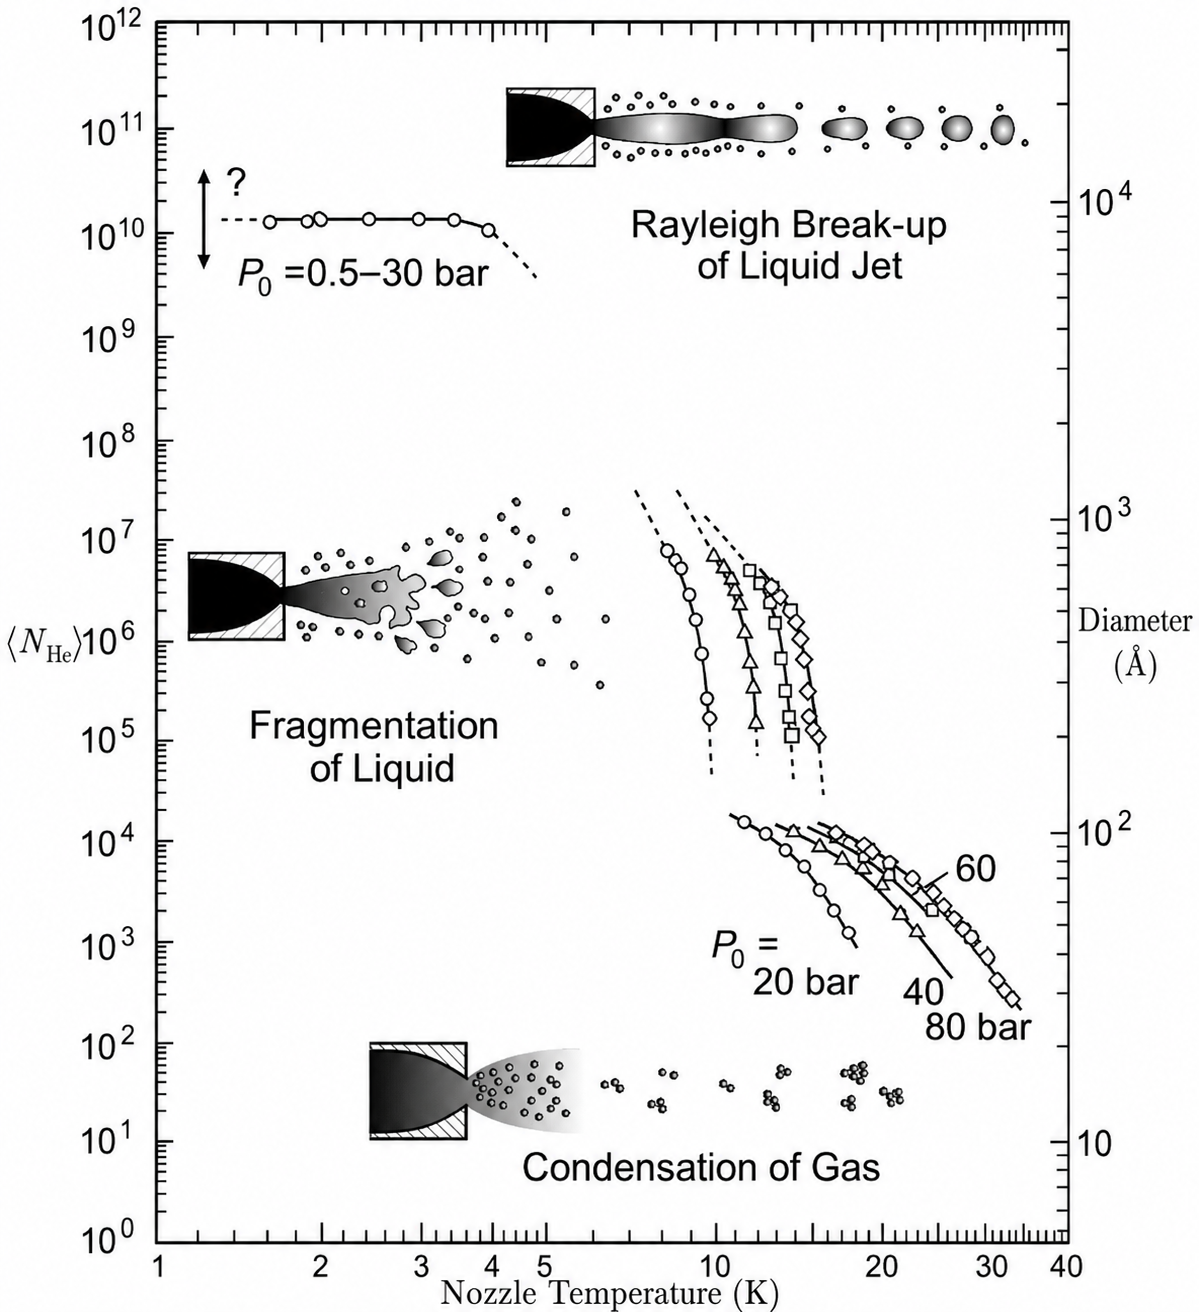
\includegraphics[width=0.8\textwidth]{03_methods/droplets.png}
    \caption{}
    \label{fig:droplets}
\end{figure}
The droplets used here are produced in the gas-condensation regime, by a continuous expansion of 30 bar helium through a \SI{5}{\micro\meter} aperture at a nozzle temperature of \SIrange{16}{18}{\kelvin}, giving $\langle N_{\mathrm{He}} \rangle \approx 3000$ atoms \cite{ianThesis}.
Once formed, the droplets cool further in vacuum by evaporation of individual helium atoms, each removing approximately \SI{5}{\per\centi\meter} (\SI{7}{\kelvin}) of internal energy. The initial cooling rate is of order 10¹⁰ K/s and decays exponentially as the droplet cools, since the evaporation rate depends exponentially on temperature. After roughly 10⁻⁴ s — far shorter than the millisecond flight time through the apparatus — evaporation becomes negligible and the temperature stabilises at 0.37 K. The droplets therefore arrive at the interaction region well below the bulk λ-point of 2.17 K and in the superfluid state.

\subsubsection{Doping Nanodroplets with Molecules}

\section{Detection and Data Acquisition}
\label{sec:detection}
\todo{}

\section{Rotating Molecules: In-Field vs Field-free}
\label{sec:rotating_molecules}
\todo{spinnability? }

%==============================================================
\chapter{In-Field Rotation of CS2 and OCS}
\label{ch:results}
%==============================================================

\section{Experimental}
\subsection{Breaking the wall}
\begin{figure}[ht]
    \centering
    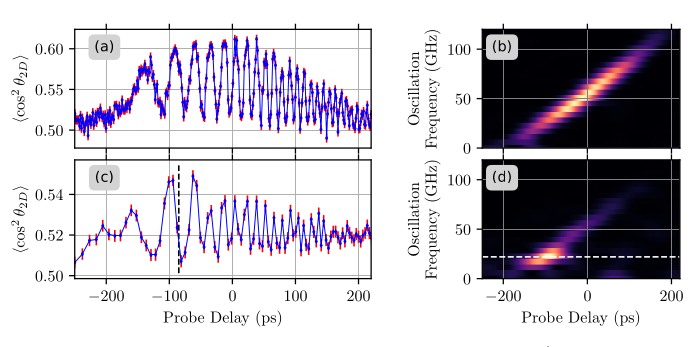
\includegraphics[width=\textwidth]{04_experiments/css_jet_and_droplets.png}
    \caption{}
    \label{fig:css_jet_and_droplets}
\end{figure}
\begin{figure}[ht]
    \centering
    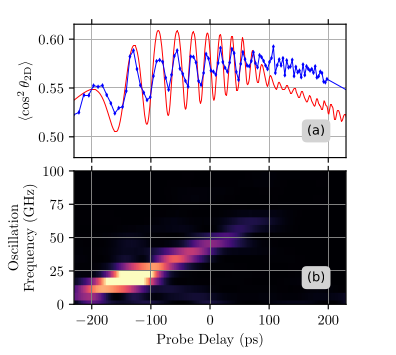
\includegraphics[width=\textwidth]{04_experiments/ocs_jet_and_droplets.png}
    \caption{}
    \label{fig:ocs_jet_and_droplets}
\end{figure}
\begin{itemize}
    \item First experiments with css and ocs -> breaking the wall
    \item explain the jet in detail: why are the oscillations so good, what are we expecting from a jet scan, clean spectrogram
    \item make insert for the spectrogram to explain what values we use
    \item Differences in css and ocs regarding their envelope and why we have a different slower centrifuge for ocs
    \item mention the other experiments with DIB and NO-Dimer
\end{itemize}

\subsection{Decelerating the molecules}
\begin{itemize}
    \item plots 
    \begin{itemize}
        \item css plot with jet decelerating and then droplets accelerating and decelerating all with spectrogram
        \item ocs the same
    \end{itemize}
    \item talk about why we did decelerating -> because the theory developed for explaining the differences between ocs and css implied independence 
    \item say what we see qualitatively 
    \item tell why it's not a surprise that the jet scans can be decelerated
    \item 
\end{itemize}
\section{Theory from Austria}

\section{Discussion}
\label{sec:discussion}
\begin{figure}[ht]
    \centering
    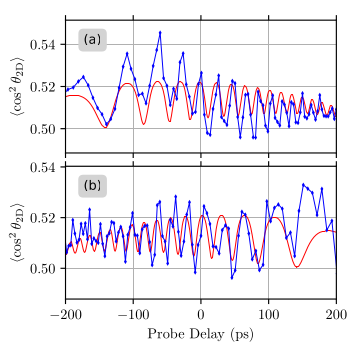
\includegraphics[width=\textwidth]{04_experiments/discussion.png}
    \caption{}
    \label{fig:discussion}
\end{figure}
\begin{itemize}
    \item plots 
    \begin{itemize}
        \item css and ocs accelerating and decelerating overlaid with the theoretical data
    \end{itemize}
\end{itemize}

%==============================================================
\chapter{Conclusion and Outlook}
\label{ch:conclusion}
%==============================================================

\section{Summary}
\label{sec:summary}
\todo{Summary of the main findings.}

\section{Outlook}
\label{sec:outlook}
\todo{Open questions and possible future experiments.}


%--- Appendix -------------------------------------------------
\appendix
%==============================================================
\chapter{Molecule Data}
\label{app:molecule_data}
%==============================================================
% ------------------------------- OCS -------------------------------
\begin{table}[htbp]
  \centering
  \caption{Rotational parameters of OCS in the gas phase and inside
           \textsuperscript{4}He nanodroplets.}
  \label{tab:ocs-params}
  \begin{tabular}{|*{6}{c|}}
    \hline
    % --- 2 cells ---
    \multicolumn{3}{|c|}{\textbf{Gas phase}} &
    \multicolumn{3}{c|}{\textbf{Helium environment}} \\
    \hline
    % --- 3 cells ---
    \multicolumn{2}{|P{\spanII}|}{%
      \pcell{$B_\mathrm{gas}$~\cite{lovas1974}}{$6.0815\,$GHz}} &
    \multicolumn{2}{P{\spanII}|}{%
      \pcell{$B_\mathrm{gas}/B_\mathrm{He}$}{$2.78$}} &
    \multicolumn{2}{P{\spanII}|}{%
      \pcell{$B_\mathrm{He}$~\cite{chatterleyRotationalCoherenceSpectroscopy2020}}{$2.19\,$GHz}} \\
    \hline
    % --- 2 cells ---
    \multicolumn{3}{|P{\spanIII}|}{%
      \pcell{$D_\mathrm{gas}$~\cite{lovas1974}}{$1.30\,$kHz}} &
    \multicolumn{3}{P{\spanIII}|}{%
      \pcell{$D_\mathrm{He}$~\cite{chatterleyRotationalCoherenceSpectroscopy2020}}{$9.5\,$MHz}} \\
    \hline
    % --- 1 cell ---
    \multicolumn{6}{|P{\spanVI}|}{%
      \pcell{$\Delta\alpha$~\cite{bridge1966}}{%
        $4.04\,\text{\AA}^3$}} \\
    \hline
    % --- 2 cells ---
    \multicolumn{3}{|P{\spanIII}|}{%
      \pcell{$\nu_\mathrm{gas}(J\!=\!0\!\to\!2)$}{$36.5\,$GHz}} &
    \multicolumn{3}{P{\spanIII}|}{%
      \pcell{$\nu_\mathrm{He}(L\!=\!0\!\to\!2)$}{$13.1\,$GHz}} \\
    \hline
  \end{tabular}
\end{table}

% ------------------------------- CS2 -------------------------------
\begin{table}[htbp]
  \centering
  \caption{Rotational parameters of CS\textsubscript{2} in the gas phase and inside
           \textsuperscript{4}He nanodroplets. Only even $J$ ($L$) are populated.}
  \label{tab:cs2-params}
  \begin{tabular}{|*{6}{c|}}
    \hline
    \multicolumn{3}{|c|}{\textbf{Gas phase}} &
    \multicolumn{3}{c|}{\textbf{Helium environment}} \\
    \hline
    \multicolumn{2}{|P{\spanII}|}{%
      \pcell{$B_\mathrm{gas}$~\cite{herzberg1966}}{$3.2715\,$GHz}} &
    \multicolumn{2}{P{\spanII}|}{%
      \pcell{$B_\mathrm{gas}/B_\mathrm{He}$}{$4.5$}} &
    \multicolumn{2}{P{\spanII}|}{%
      \pcell{$B_\mathrm{He}$~\cite{chatterleyRotationalCoherenceSpectroscopy2020}}{$0.72\,$GHz}} \\
    \hline
    \multicolumn{3}{|P{\spanIII}|}{%
      \pcell{$D_\mathrm{gas}$~\cite{herzberg1966}}{$\approx 0.4\,$kHz}} &
    \multicolumn{3}{P{\spanIII}|}{%
      \pcell{$D_\mathrm{He}$~\cite{chatterleyRotationalCoherenceSpectroscopy2020}}{$0.9\,$MHz}} \\
    \hline
    \multicolumn{6}{|P{\spanVI}|}{%
      \pcell{$\Delta\alpha$~\cite{bridge1966}}{%
        $\approx 9.6\,\text{\AA}^3$}} \\
    \hline
    \multicolumn{3}{|P{\spanIII}|}{%
      \pcell{$\nu_\mathrm{gas}(J\!=\!0\!\to\!2)$}{$19.6\,$GHz}} &
    \multicolumn{3}{P{\spanIII}|}{%
      \pcell{$\nu_\mathrm{He}(L\!=\!0\!\to\!2)$}{$4.3\,$GHz}} \\
    \hline
  \end{tabular}
\end{table}
% Supplementary derivations, extended data tables, additional figures.
\todo{Find citations and add ratio of D}

\begin{table}[htbp]
  \centering
\caption{Rotational parameters of the nitric oxide dimer, \textit{cis}-ONNO,
in the gas phase and inside \textsuperscript{4}He nanodroplets.}
\label{tab:no2-params}
\begin{tabular}{|*{6}{c|}}
\hline
% --- 2 cells ---
\multicolumn{3}{|c|}{\textbf{Gas phase}} &
\multicolumn{3}{c|}{\textbf{Helium environment}} \\
\hline
% --- 3 cells ---
\multicolumn{2}{|P{\spanII}|}{%
\pcell{$B_{yz}^\mathrm{gas}$~\cite{howard1993}}{$5.10\,$GHz}} &
\multicolumn{2}{P{\spanII}|}{%
\pcell{$B_{yz}^\mathrm{gas}/B_{yz}^\mathrm{He}$}{$1.9$}} &
\multicolumn{2}{P{\spanII}|}{%
\pcell{$B_{yz}^\mathrm{He}$~\cite{macphail-bartleyControlMolecularRotation2026a}}{$2.76(6)\,$GHz}} \\
\hline
% --- 2 cells ---
\multicolumn{3}{|P{\spanIII}|}{%
\pcell{$D_\mathrm{gas}$~\cite{howard1993}}{%
$\approx 1\times10^{-6}\,$cm\textsuperscript{-1}}} &
\multicolumn{3}{P{\spanIII}|}{%
\pcell{$D_\mathrm{He}$}{---}} \\
\hline
% --- 1 cell ---
\multicolumn{6}{|P{\spanVI}|}{%
\pcell{$\Delta\alpha$~\cite{cccbdb} (calculated)}{%
$3.4\,\text{\AA}^3$}} \\
\hline
% --- 2 cells ---
\multicolumn{3}{|P{\spanIII}|}{%
\pcell{$\nu_\mathrm{gas}(J\!=\!0\!\to\!2)$}{$31\,$GHz}} &
\multicolumn{3}{P{\spanIII}|}{%
\pcell{$\nu_\mathrm{He}(J\!=\!0\!\to\!2)$}{$16.8(4)\,$GHz}} \\
\hline
\end{tabular}
\end{table}

\chapter{Different molecules/ experiments}


\chapter{Useful information when conducting experiments}
\section{Chamber Pressures}
\subsection{Vacuum setup}
\section{Optical alignment}
\section{Switching between Jet and Droplets}
\section{Finding the correct TOF window}


\chapter{AI-generated content}
\label{sec:ai}
Content wise, artificial intelligence was only used in the theoretical background section \ref{sec:theory}, with the purpose of accelerating and enhancing the explanation of already known science and math. Every result, if not marked different, was checked and verified by me. Places where AI altered results are used, have footnote markings. 

\section{Numerical illustration of rotational ladder climbing}
\label{app:centrifuge-tdse}
For the purpose of displaying the rotational ladder climbing mechanism, I used Claude to write a script that simulates the dynamics of the rotating frame Hamiltonian \eqnref{eq:rotating_frame_hamiltonian}. This code is \textbf{not} proofread by me, but sanity checked through the outcomes of the simulation.  It implements a direct
numerical solution of the time-dependent Schr\"odinger equation (TDSE) for a rigid rotor driven by an optical centrifuge. The intention of this calculation is of pedagogical nature: it is used to generate the figures that show how population is transferred stepwise up the rotational ladder, and it is not presented as a quantitative model of the experiment reported in this work.

The following explanation of the code is generated by AI.

\subsection{Physical model}
\label{app:centrifuge-model}

The optical centrifuge is formed from two counter-rotating, counter-chirped circularly polarised beams, whose superposition is a linearly polarised field
whose polarisation direction $\phi_d(t)$ rotates with increasing angular
velocity. After averaging over the optical carrier, a linear molecule of
polarisability components $\alpha_\parallel,\alpha_\perp$ experiences the
interaction
%
\begin{equation}
  V(t) = -\frac{\varepsilon_0^2(t)}{4}
         \left[\alpha_\perp
               + \Delta\alpha\,\sin^2\theta\,\cos^2\!\bigl(\varphi-\phi_d(t)\bigr)\right],
  \qquad \Delta\alpha = \alpha_\parallel-\alpha_\perp ,
  \label{eq:app-lab-interaction}
\end{equation}
%
where $\theta,\varphi$ are the polar and azimuthal angles of the molecular
axis and $\varepsilon_0(t)$ is the field envelope. Transforming to the frame
co-rotating with the polarisation by means of the unitary operator
$\hat U(t)=\exp[-\mathrm{i}\phi_d(t)\hat J_z]$ removes the explicit
$\phi_d$-dependence at the cost of an inertial term, giving the working
Hamiltonian
%
\begin{equation}
  \hat{\tilde H}(t)
  = B\hat J^{2}
    - \hbar\Omega(t)\hat J_{z}
    - \frac{\varepsilon_0^2(t)}{4}
      \bigl[\alpha_\perp + \Delta\alpha\,\sin^2\theta\cos^2\varphi\bigr],
  \qquad \Omega=\dot\Phi .
  \label{eq:app-rotating-frame}
\end{equation}
%
This change of frame is exact; no approximation is involved, and no
restriction is placed on $\dot\Omega$. Two further points about
Eq.~\eqref{eq:app-rotating-frame} as implemented:

\begin{enumerate}
  \item The isotropic term $-\tfrac{1}{4}\varepsilon_0^2\alpha_\perp$ is
        proportional to the identity operator. It therefore contributes only a
        time-dependent global phase and cannot affect any observable. It is
        omitted from the computation.
  \item Writing $U(t)=\Delta\alpha\,\varepsilon_0^2(t)/4$ and
        $\Omega(t)=2\pi f_d(t)$, the propagated Hamiltonian in frequency units
        is
        \begin{equation}
          \tilde H(t)/h = B\,J(J+1) - f_d(t)\,M - \frac{U(t)}{h}\,Q_x,
          \qquad Q_x \equiv \sin^2\theta\cos^2\varphi .
          \label{eq:app-working-hamiltonian}
        \end{equation}
\end{enumerate}

\paragraph{Basis.}
The wavefunction is expanded in field-free rigid-rotor eigenstates
$\ket{J,M}$. Because $Q_x$ is a rank-2 spherical tensor with components
$q=0,\pm2$, it obeys the selection rules $\Delta J=0,\pm2$ and
$\Delta M=0,\pm2$ and therefore conserves the parity of both $J$ and $M$.
Starting from $\ket{0,0}$, the accessible Hilbert space is exactly the set of
states with even $J$ and even $M$; restriction to this sector is a rigorous
symmetry reduction rather than an approximation. The basis is truncated at
$J_{\max}$, giving $81$ states for $J_{\max}=16$.

The interaction matrix is built from the spherical-harmonic expansion
%
\begin{equation}
  Q_x = \frac{1}{3}
        - \sqrt{\frac{4\pi}{45}}\,Y_2^{0}
        + \sqrt{\frac{2\pi}{15}}\left(Y_2^{2}+Y_2^{-2}\right),
  \label{eq:app-qx-expansion}
\end{equation}
%
with matrix elements evaluated in closed form from Wigner $3j$ symbols,
%
\begin{equation}
  \begin{aligned}
  \braket{J'M'|Y_k^q|JM}
  \\= (-1)^{M'}\sqrt{\frac{(2J'+1)(2k+1)(2J+1)}{4\pi}}
    \begin{pmatrix} J' & k & J\\ 0&0&0\end{pmatrix}
    \begin{pmatrix} J' & k & J\\ -M' & q & M\end{pmatrix}.
  \end{aligned}
  \label{eq:app-wigner}
\end{equation}
%
Both the $q=+2$ and $q=-2$ terms are retained. The calculation therefore makes
\emph{no} rotating-wave approximation and imposes \emph{no} constraint
$M=J$; couplings that violate the resonant selection rule $\Delta J=\Delta M$
are present, as are all $\Delta J=0$ (dressing) terms.

\paragraph{Pulse and chirp schedule.}
The laser intensity envelope is Gaussian with full width at half maximum
$\tau_{\mathrm{FWHM}}$, centred at $t=0$; since the polarisability interaction
is linear in intensity,
%
\begin{equation}
  U(t)/h = (U_0/h)\,\exp\!\left[-4\ln 2\,(t/\tau_{\mathrm{FWHM}})^2\right].
  \label{eq:app-envelope}
\end{equation}
%
The rotation frequency is held at zero, ramped linearly across the FWHM
interval, and then held constant:
%
\begin{equation}
  f_d(t) = f_{\mathrm{final}}\times
  \begin{cases}
    0, & t \le -\tau_{\mathrm{FWHM}}/2,\\[2pt]
    \bigl(t+\tau_{\mathrm{FWHM}}/2\bigr)/\tau_{\mathrm{FWHM}},
      & |t| < \tau_{\mathrm{FWHM}}/2,\\[2pt]
    1, & t \ge +\tau_{\mathrm{FWHM}}/2 .
  \end{cases}
  \label{eq:app-chirp}
\end{equation}
%
The field is thus already at half its peak value when the rotation begins, so
the molecule is adiabatically dressed into a pendular state before the
centrifuge starts, and the field is still at half peak when the rotation stops,
so the final state is released by a slow turn-off at constant $\Omega$. Each
value of $f_{\mathrm{final}}$ corresponds to a different constant angular
acceleration.

Propagation begins and ends where $U/U_0=10^{-4}$ rather than at the edges of
the plotted window, so that the initial condition $\ket{0,0}$ is imposed in an
essentially field-free region and the reported final populations are
field-free populations rather than populations of dressed states. Because the
frame transformation is diagonal in $M$ and does not mix $J$, the quantities
$P_J$ and $\langle J\rangle$ are identical in the rotating and laboratory
frames.

\subsection{Numerical method and parameters}
\label{app:centrifuge-numerics}

The TDSE is integrated with a symmetric (Strang) split-operator propagator,
%
\begin{equation}
  \exp\!\left[-\tfrac{\mathrm{i}}{\hbar}\tilde H\,\delta t\right]
  \simeq
  \mathrm{e}^{-\mathrm{i}\tilde H_{\mathrm{diag}}\delta t/2\hbar}\,
  \mathrm{e}^{-\mathrm{i}\tilde H_{\mathrm{int}}\delta t/\hbar}\,
  \mathrm{e}^{-\mathrm{i}\tilde H_{\mathrm{diag}}\delta t/2\hbar}
  + \mathcal{O}(\delta t^{3}),
  \label{eq:app-strang}
\end{equation}
%
where $\tilde H_{\mathrm{diag}}/h = B J(J+1) - f_d(t)M$ is diagonal in
$\ket{J,M}$ and $\tilde H_{\mathrm{int}}/h = -(U(t)/h)\,Q_x$ is diagonal in the
eigenbasis of $Q_x$. Since $Q_x$ is time-independent, it is diagonalised once
and reused. Each factor is separately unitary. All values of
$f_{\mathrm{final}}$ are propagated simultaneously as columns of a single
matrix; this is mathematically identical to independent runs.

Parameters are collected in Table~\ref{tab:app-parameters}.

\begin{table}[htbp]
  \centering
  \caption{Parameters of the ladder-climbing calculation.}
  \label{tab:app-parameters}
  \begin{tabular}{llll}
    \toprule
    Quantity & Symbol & Value & Source / note \\
    \midrule
    Rotational constant & $B$ & \SI{6.081492}{\giga\hertz}
      & gas-phase $B_0$ of $^{16}$O$^{12}$C$^{32}$S \\
    Centrifugal distortion & $D$ & --- & omitted \\
    Polarisability anisotropy & $\Delta\alpha$ & \SI{5.34}{\cubic\angstrom}
      & static value \\
    Peak intensity & $I_0$ & \SI{1e11}{\watt\per\square\centi\meter} & \\
    Peak coupling & $U_0/h$ & \SI{168.9}{\giga\hertz} & derived \\
    Dimensionless coupling & $U_0/B$ & $27.8$ & derived \\
    Intensity FWHM & $\tau_{\mathrm{FWHM}}$ & \SI{320}{\pico\second} & \\
    Final frequency range & $f_{\mathrm{final}}$ & $0$--\SI{120}{\giga\hertz}
      & 200 values \\
    Basis truncation & $J_{\max}$ & $16$ & 81 states \\
    Integration step & $\delta t$ & \SI{0.05}{\pico\second} & \\
    Initial state & --- & $\ket{J=0,M=0}$ & $T=\SI{0}{\kelvin}$ \\
    \bottomrule
  \end{tabular}
\end{table}

\subsection{Verification}
\label{app:centrifuge-verification}

The following checks were performed and are reported here so that the
calculation can be reproduced or refuted.

\begin{enumerate}
  \item \textbf{Operator construction.} The diagonal element
        $\braket{0,0|Q_x|0,0}$ reproduces the analytic spherical average
        $\langle\sin^2\theta\cos^2\varphi\rangle = 1/3$ to machine precision,
        and all eigenvalues of the truncated $Q_x$ matrix lie within the range
        $[0,1]$ of the exact operator.
  \item \textbf{Time-step convergence.} Reducing $\delta t$ by a factor of
        four changes the final $\langle J\rangle$ in the seventh decimal
        place. Note that norm conservation is \emph{not} a useful convergence
        diagnostic here, because the split propagator is unitary by
        construction; the norm is conserved to roundoff regardless of whether
        $\delta t$ is adequate.
  \item \textbf{Basis convergence.} Increasing $J_{\max}$ from 16 to 24 leaves
        the final populations unchanged to six decimal places. The population
        residing in the highest retained $J$ manifold remains below $10^{-12}$
        throughout.
  \item \textbf{Consistency with the analytic ladder picture.} The final
        rotational state agrees with the number of two-photon resonances
        $f_d = B(2J+3)$ traversed during the chirp, and simultaneously with the
        classical trapped-rotor estimate $J\approx f_d/2B$; at these parameters
        the two predictions coincide. Representative values are given in
        Table~\ref{tab:app-results}.
  \item \textbf{Role of non-resonant couplings.} At these parameters
        $99.99\,\%$ of the final population lies in the chain
        $C\equiv J-M=0$, and imposing the rotating-wave approximation by hand
        changes the final populations by $<10^{-3}$. The non-resonant terms are
        thus retained but numerically inactive here; their inclusion matters
        for weaker fields or thermal initial conditions.
\end{enumerate}

\begin{table}[htbp]
  \centering
  \caption{Representative results. $\sigma_J$ is the standard deviation of the
           final rotational distribution.}
  \label{tab:app-results}
  \begin{tabular}{S[table-format=3.0] S[table-format=2.3] S[table-format=1.2] S[table-format=1.3]}
    \toprule
    {$f_{\mathrm{final}}$ (GHz)} & {$\langle J\rangle_{\mathrm{final}}$}
      & {$\sigma_J$} & {$P_{J_{\mathrm{dom}}}$} \\
    \midrule
     60 &  4.002 & 0.07 & 0.999 \\
    100 &  7.991 & 0.14 & 0.995 \\
    120 &  9.986 & 0.18 & 0.993 \\
    \bottomrule
  \end{tabular}
\end{table}

At the parameters of Table~\ref{tab:app-parameters} the transfer is close to
adiabatic: more than $99\,\%$ of the population ends in a single rotational
state with $\sigma_J\lesssim0.2$. In the dimensionless parametrisation of
Armon and Friedland \cite{armonQuantumClassicalDynamics2017}, the calculation sits near
the boundary between quantum ladder climbing and classical autoresonance
($P_1\approx15$, $P_2\approx1.1$ at the largest final frequency), with the
autoresonant capture criterion $P_1P_2>1/2$ satisfied by more than an order of
magnitude. Weaker fields or faster chirps move the system towards the
non-adiabatic regime, in which population is left behind at successive
crossings and the final distribution broadens.

\subsection{Limitations}
\label{app:centrifuge-limitations}

The following are omitted from the model and bound its interpretation.

\begin{itemize}
  \item \textbf{Centrifugal distortion.} The rotor is treated as rigid. The
        correction to the two-photon resonance grows as $J^{3}$ and is
        negligible over the range of $J$ shown here, but the model must not be
        extrapolated to superrotor states without reinstating $D$.
  \item \textbf{Temperature.} The calculation starts from the single pure
        state $\ket{0,0}$. A thermal ensemble populates many initial
        $\ket{J_0,M_0}$, which are captured into the rotating well with
        differing efficiency; the resulting bifurcation between trapped and
        untrapped populations is the dominant source of the broad final
        distributions seen experimentally, and it is absent here by
        construction.
  \item \textbf{Polarisability.} The static $\Delta\alpha$ is used in place of
        the frequency-dependent value at the laser wavelength.
  \item \textbf{Experimental averaging.} No focal-volume or intensity
        averaging is performed; a single peak intensity is assumed.
  \item \textbf{Dissipation.} The propagation is strictly unitary. Collisional
        and environmental decoherence are not included.
\end{itemize}

%--- Bibliography ---------------------------------------------
\cleardoublepage
\printbibliography[heading=bibintoc]

%--- Back matter ----------------------------------------------
%==============================================================
%  Acknowledgements
%==============================================================
\chapter*{Acknowledgements}
\addcontentsline{toc}{chapter}{Acknowledgements}

\todo{Acknowledgements.}

\cleardoublepage
%==============================================================
%  Declaration of authorship / Eidesstattliche Erklaerung
%  (adapt wording to your institution's exact template)
%==============================================================
\chapter*{Declaration of Authorship}
\addcontentsline{toc}{chapter}{Declaration of Authorship}

I hereby declare that this thesis is my own work and that I have used no
sources or aids other than those indicated. All passages taken verbatim
or in substance from published or unpublished sources are marked as such.
This thesis has not been submitted, in the same or a similar form, to any
other examination authority.

\vspace{2.5cm}

\noindent
\begin{tabular}{@{}p{6cm}p{6cm}@{}}
\hrulefill & \hrulefill \\
Place, Date & Signature \\
\end{tabular}


%==============================================================
\end{document}
%==============================================================
